
%
%  $Description: Author guidelines and sample document in LaTeX 2.09$ 
%
%  $Author: ienne $
%  $Date: 1995/09/15 15:20:59 $
%  $Revision: 1.4 $
%

\documentclass[times, 10pt,twocolumn]{article} 
\usepackage{amsmath}
\usepackage{latex8}
\usepackage{algorithmic}
\usepackage{algorithm}
\usepackage{amsfonts}
\usepackage{subfigure}
\usepackage{amssymb}
\usepackage[small]{caption}
 \usepackage{graphicx}
\usepackage{amsmath}
\usepackage{multirow}
\usepackage{comment}
\usepackage{enumerate}
\usepackage{latexsym}
\usepackage{tipa}

\usepackage{times}
\newcommand{\bs}[0]{\textrm{\textbackslash}}
\newcommand{\clique}[1]{\vec #1_{\{k\}}}

\DeclareMathOperator*{\unif}{Unif}

%\documentstyle[times,art10,twocolumn,latex8]{article}

%------------------------------------------------------------------------- 
% take the % away on next line to produce the final camera-ready version 
\pagestyle{empty}

%------------------------------------------------------------------------- 
\begin{document}

\title{An Investigation into Concurrent Expectation Propagation}

\author{David Hall and Alex Kantchelian \\
EECS CS Division \\ University of California, Berkeley\\ \texttt{\{dlwh,
akant\}@cs.berkeley.edu}\\
}

\maketitle
\thispagestyle{empty}

\begin{abstract}
As statistical machine learning becomes more and more prevalent and models become more complicated and fit to larger amounts of data, approximate inference mechanisms become more and more crucial to their success. Expectation propagation (EP) is one such algorithm for inference in probabilistic graphical models. In this work, we introduce a robustified version of EP which helps ensure convergence under a relaxed memory consistency model. The resulting algorithm can be efficiently implemented on a GPU in a straightforward way. Using a 2D Ising spin glass model, we evaluate both the original EP algorithm and our robustified version in terms of convergence, if any, and precision on a classic single core processor. We also compare the naive parallelized version of the original EP algorithm against the parallelized robustified EP on both a multicore CPU and a GPU.
\end{abstract}



\section{Introduction}

Probabilistic graphical models (PGMs) are one of the cornerstones
of modern AI, with applications ranging from medical diagnosis, to
social network analysis, to robotics. PGMs provide the flexibility
to model almost any real world phenomena in a coherent, simple way.
However, exact computation in all but the most trivial PGMs is
impossible. In the discrete case, inference in PGMs is
\#P-complete~\cite{Koller2009pgm}, and for continuous variables it is
possible to come up with incomputable models, even for ``well
behaved'' distributions~\cite{AFR11}.

Therefore, approximate inference regimes are one of the main cottage
industries within the AI community, with several variants proposed
each year. Broadly, they fall into three categories. The first is
based on random sampling, especially Markov Chain Monte Carlo. MCMC
is a randomized algorithm that is perhaps the easiest to implement,
though it almost always the slowest in practice. Second are relaxation
techniques based on linear or convex programming, but these are
complex to implement and require significantly different implementations
for each new PGM considered. Finally, there are message passing
algorithms like mean field inference, belief propagation, and
expectation propagation.  We focus on message passing algorithms.

Unfortunately, all of these algorithms are tricky to parallelize,
especially on arbitrarily structured graphs. Most of these algorithms
can be parallelized to a certain extent given a graph coloring, but
there is a limit to how much parallelism can be extracted from graph
partitions in arbitrary graphs.

Message passing algorithms such as Expectation
Propagation~\cite{Minka01} optimize an approximation to the true
PGM that is ``as close as possible'' to the original graph while
remaining within a tractable set of decomposed distributions.
Operationally, these algorithms typically work by decomposing the
graph structure into subgraphs, and then (potentially) further
approximating those parts with simpler distributions. Then, one
component is updated at a time, optimizing it locally using the
other components as a guide. That is, these algorithms are basically
a kind of coordinate ascent. This implies that these updates are
inherently sequential: coordinate ascent only makes sense if one
coordinate is updated at a time.

However, it is possible to just perform these updates in parallel,
using ``old information'' when making decisions~\cite{CsekeHeskes2010}.
However, this update schedule can exacerbate the non-convergence
problems already observed in practice. Because there are multiple
local optima, different components of the graph might be attracted
to different optima, leading to oscillations.

We propose a new message passing algorithm called Convex Expectation
Propagation (CEP) that allows for non-serialized concurrent updates
without introducing the same pathologies possible in the na\"ive
algorithm.  One class of approximations---convex approximations---ensures
that there is only one optimum\cite{wainwright03trw}. Thus, different
pieces of the structure of the graph (which are operating largely
independently on different processors) cannot update towards different
local optima, which is one of the primary sources of oscillation.

We implemented CEP on both a CPU and a commodity GPU, via the new
OpenCL standard. We compare our algorithm to a serialized version
of the algorithm, as well as a non-robustified traditional version
of EP. We consider three metrics: accuracy, speed, and convergence.
We show that while EP performs surprisingly well in many circumstances
even when parallelized, it does for some conditions exhibit the
oscillations and slower convergence we hypothesized. Moreover, our
new algorithm does not exhibit these problems, though it usually
less accurate. We therefore consider an unprincipled compromise
between the two algorithms, finding that it combines the benefits of
both algorithms.

This paper is organized as follows. First, we describe necessary
background on probabilistic graphical models. Second, we describe
Expectation Propagation. Third, we motivate and present Convex
Expectation Propagation. Then, we conduct our experiments on
synthetic models in a Ising spin-glass model under a variety of
parameter conditions. Finally, we discuss potential future avenues
for research.

\section{Graphical Models}
\begin{figure}[t]
  \centering
  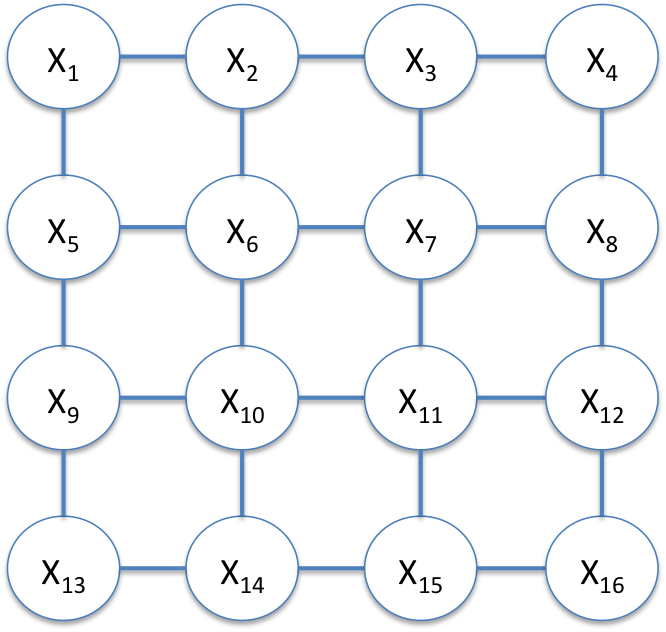
\includegraphics[scale=0.6]{ising.png}
  \caption{A 2-D Ising model, a commonly employed synthetic class of
  graphical model. Ising models are pairwise graphical models over
  binary-valued random variables with
  two kind of potentials: singleton and pair. Singleton potentials
  govern the probability a variable is ``on'' in isolation, while
  the pairwise potentials govern the extent to which variables
  agree or disagree with their neighbors.}
  \label{fig:ising}
\end{figure}

Probabilistic graphical models are defined on a graph structure as
in Figure \ref{fig:ising}.\footnote{We focus on the undirected case.
These are sometimes called Markov Random Fields.} Each PGM defines
a class of probability distributed that share certain independence
assumptions.  The nodes in a graph are the underlying random variables,
and a variable is independent of all other variables conditioned on
observations about all of its neighbors. For instance, in Figure
\ref{fig:ising}, $X_1$ is independent of all other variables given
$X_2$ and $X_5$.

A graphical model does not describe a single probability distribution.
Instead, we need a set of \textit{potential functions} $\psi$, possibly
one for each clique $\clique{x}$ in the underlying graph:
\begin{equation}
  \begin{split}
    p(x_1, \ldots, x_n) &= \frac1Z \prod_{k} \psi_k(\clique{x}) \\
    Z &= \sum_{x'_1, \ldots, x'_n} \prod_{k} \psi_k(\clique{x'})
   \end{split}
   \label{eqn:prob}
 \end{equation}
$Z$ is called the partition function and ensures the distribution
normalizes to unity. Note that it involves a sum over all possible
assignments to all variables, which can take exponential time in an
arbitrary graph. Most of our attention will be focused on
approximating this term.

Usually, for both theory and practice, it is convenient to
represent these distributions in the exponential family of
distributions as follows:
\begin{equation}
  \begin{split}
    p(x_1, \ldots, x_n) &= \exp\left ( \sum_{k} \langle \theta_k,
    \phi^k(\clique{x}) \rangle - A(\theta) \right ) \\
    A(\theta) &= \log \sum_{x'_1, \ldots, x'_n}  \exp\left (
    \sum_{k} \langle \theta_k, \phi^k(\clique{x'}) \rangle \right )
   \end{split}
 \end{equation}
Each $\phi^k(\cdot)$ is a ``feature'' or ``projection'' function
that lifts the underlying variables in a space where the potential
function can be computed as the exponentiation of an inner product.
$A(\theta)$ is called the log-partition function.

In this paper, we actually restrict ourselves to pairwise graphical models:
models where the potentials are constrained to at most 2 variables.
That is, we consider models of the form:
\begin{equation}
  \begin{split}
    p(x_1, \ldots, x_n)  &= \frac1Z \prod_i \psi_i(x_i) \prod_{i,j}
    \psi_{ij}(x_i, x_j) \\
   \end{split}
   \label{eqn:pairwise}
 \end{equation}
Arbitrary graphical models can be made pairwise via a simple
transform, and so it is appropriate for simulation studies. In
particular, we use the Ising Model for our experiments. Everything
we find should generalize to higher arity models.


There are two \textit{inference} tasks commonly associated with
graphical models. The first is the identification of the maximum
probability assignment to all variables. The second is the task of
determining the partition function $Z$ or marginal distributions
$\mu(x_i, x_j, \ldots)$.  For general discrete distributions, this
first task is NP-hard, while the second task is \#P-hard in the
general case.

Many papers have been written on methods for approximately solving
both of these problems, as well as identifying subclasses of PGMs
where one or the other task is tractable. (See, e.g.,
\cite{taskar03m3n})
In this paper, we focus on the second, harder, task, choosing to
study in particular on Expectation Propagation\cite{Minka01}.

\section{Expectation Propagation}
\begin{figure}
\centering
	\subfigure[Fully disconnected ``core''
  graph]{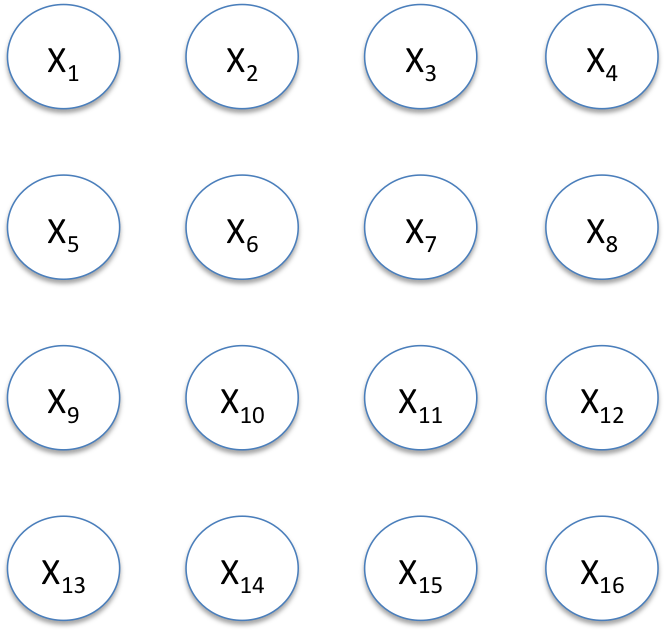
\includegraphics[scale=0.4]{ising-discon.png}}
  \subfigure[An ``augmented'' graph with one
  edge]{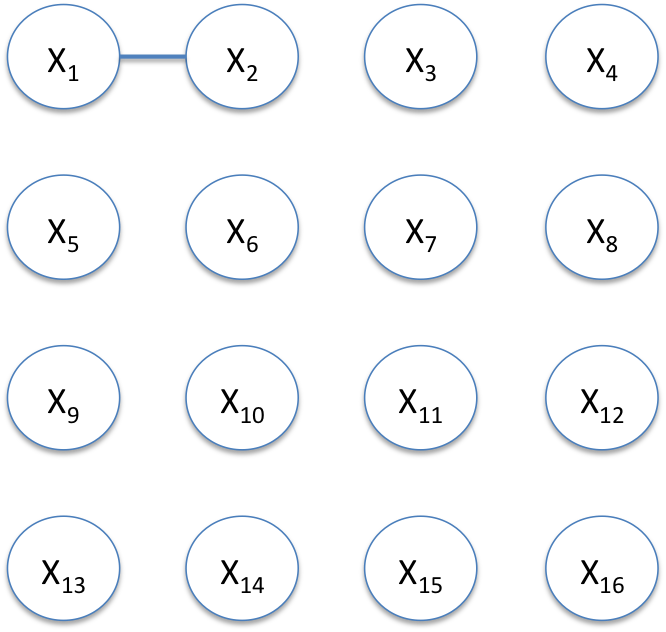
\includegraphics[scale=0.4]{ising-one-con.png}}
  \caption{EP functions by using a ``core'' graph and a collection
  of ``augmented'' graphs. The goal is to approximate the original
  connected graph (like in Figure \ref{fig:ising}) with the fully
  disconnected graph, by augmenting the graph one at a time, and
  iteratively ``projecting'' this augmented graph down to the
  original core graph.}
  \label{fig:ep}
\end{figure}

Recall in our discussion of Equation \ref{eqn:prob} that the
exponential number of assignments to the variables $x_1,\ldots,x_k$
was the source of the intractability associated with inference in
graphical models. If, however, our graph is suitably structured---say,
a fully disconnected graph or a tree---then computing this sum would
be possible in polynomial time via dynamic programming. Moreover,
if a graph structure is just ``a little intractable'' then inference
is still not so bad. For instance, a graph with a single loop can
be decomposed into just a few trees by summing over the loop in the
outermost layer of the sum. More generally, if we could find a way
to efficiently approximate a full graph by a ``simple graph'' and a
collection of ``slightly intractable'' graphs, we could perform the
sum efficiently.

Expectation Propagation\cite{Minka01} seeks to operationalize this
intuition precisely. Define a core graph by a feature function
$\phi^0$ that collects some subset of the original feature
functions. For instance, in the Ising model in Figure
\ref{fig:ising}, we might choose the potentials on the fully
disconnected graph in Figure \ref{fig:ep}a. Then, we cluster the
remaining potentials into ``augmented'' graphs. For instance, we
might keep each edge in its own cluster, as in Figure
\ref{fig:ep}b. Denote these clusters by their clustered feature
functions $\phi^i$.

EP works by taking the potentials from an augmented graph and
combining them with an ``adjusted'' version of the core graph.
Specifically, we maintain a distribution $q$ based on the core graph
that approximates $p$ as closely as possible. At each step, we
choose an augmented graph with features $\phi^k$, multiply it in
with $q$ (after removing cluster $k$'s contribution to q), and then
create a new $q$ that looks as much like the product as possible.
Write the potentials associated with the augmented graph by $f_k(x)
= \exp( \langle \theta^k, \phi^k(x) \rangle )$, and let
$\tilde f_k(x) = \exp( \langle \lambda_k, \phi^0(x)\rangle$ be
$f_k$'s contribution to the $q$. The algorithm is as follows:
\begin{enumerate}
  \item Initialize the $\tilde f_k$.
  \item Set $q(x) \propto \prod_k \tilde f_k$.
  \item Until convergence, choose $k$:
  \item Create $q^{\bs k}(x) = q(x) / \tilde f_k(x)$
  \item Create the augmented distribution:\\
    $q_k(x) = q^{\bs
    k}(x)\cdot f_k(x)$.
  \item Project $\mathrm{KL}(q_k(x) || q^{\textrm{new}}(x))$
  \item Store $\tilde f_k(x) = q^{\textrm{new}}(x)/q(x)$
\end{enumerate}
Step 6 simply says that one should adjust $q$ to have the same
expectations as $q_k$ for all of the features in $\phi^0$. For
instance, if we use a fully disconnected graph as our $q$, then we
will update $q$ so that the marginal distributions $\mu_i(x_i)$
will be the same in both graphs.

From a practical perspective, this algorithm is much easier to
implement than it looks. Note that all of these functions are just
the exponentiation of dot products. Therefore, the multiplication
of two terms just the addition of two vectors (say $\theta^0$ and
$\lambda_k$), while division is just subtraction. 

Finally, EP is defined sequentially, but one could perform the
updates in parallel, simply computing the $\tilde f_k$ in parallel and
reconstituting $q$ in a reduce-scatter operation. 

\section{Convex Expectation Propagation}

Like almost all message-passing-based approximate inference algorithms, EP is known to
have multiple local optima. (The main exception to our knowledge
is Tree-Reweighted Belief Propagation~\cite{wainwright03trw}.) In practice, sequential EP seems to have little
issue with these local optima, as the errors found with EP are
typically much lower than with other algorithms. Moreover, the
algorithm always seems to converge.

However, when doing parallel updates, EP is basically using
``stale'' information. That is, when doing each update, the
different components have no knowledge of the changes about to be
performed by the other graphs. Because different subgraphs might
be locally attracted to different optima, we claim that
parallel-update EP is less likely to converge, because it might
alternate between these optima. 

The reason that Tree-Reweighted Belief propagation is exempted from
this critique is that it attempts to optimize a \textit{convex}
relaxation of the objective function. Convexity assures, among many
other things, that there is at most one optimum.\footnote{In principle
the optimum could be at $\pm\infty$.} Thus, even if the updates in
the Tree-Reweighted case are done in parallel, they cannot be
attracted to different local optima because they simply do not
exist.

We propose, therefore, to modify EP by ``convexifying'' its updates.
Here, we derive the algorithm starting from the modified objective
function. Our proof---given sufficient background---is fairly
straightforward, and follows the derivation of standard EP given in
\cite{wainwright08graphical} closely.

\subsection{The EP Objective}

We begin by motivating the EP objective function. First, we use standard results to rewrite the log-partition
function $A(\theta)$:
\begin{equation}
  \begin{split}
     A(\theta) &= \log \sum_x \langle\theta,\phi(x)\rangle\\
     &= \max_{\mu \in \mathcal{M}} \{ \langle\theta,\mu\rangle + H(\mu) \}
   \end{split}
 \end{equation}
with summation replaced by integration as appropriate. Here, $\mu$
is a function defining marginal distributions and $H$ is the standard
entropy functional in base $e$. There are two problems to computing
this function directly. First, there are potentially exponentially
many constraints defining the set $\mathcal M$. Second, the term
$H(\mu)$ might not decouple in a way that admits efficient dynamic
programming. We will relax both of these conditions.

First, we split the graphical model with features $\phi$ into
a number of components. Specifically, there are the \textit{core}
features $\phi^0$, and then a set of \textit{augmented}
features $\phi^i$. In the Ising model, the core features would
be the singleton potentials, while the $\phi^i$ correspond to
non-overlapping subsets of the various edges. Clearly, taking all
of these features together yields the original model, while taking
just the core features and one of the $\phi^i$ yields 
a relaxed approximation to the full model, which we will call an
\textit{augmented} model.

The key insight behind standard EP is to approximate the entropy of
the full model as follows:
\begin{equation}
  \begin{split}
     H(\mu) &\approx H(\mu^0) + \sum_i \left ( H( (\mu^0,\mu^i)) -
     H(\mu^0)\right) \\
     & \stackrel{\Delta}= F(\mu^0, \ldots, \mu^n) \\
     \label{eqn:epentropy}
   \end{split}
 \end{equation}
Intuitively, this expression says that the full entropy function
$H$ can be approximated as the entropy of the core model, plus
a set of ``corrections'' from each of the augmented models.

What remains is to relax the set $\mathcal M$ to one with fewer
constraints. This can be achieved by specifying that each of the
marginals $(\mu^0,\mu^0)$ must live in a set $\mathcal M^i$ that
specifies constraints that affect only the variables and potentials
used in that augmented model. All together, we obtain a new
objective:
\begin{equation}
  \begin{split}
     A(\theta) 
     &\approx \max_{(\mu^0,\mu^i) \in \mathcal{M}^i} \{ \langle
     \theta^0, \mu^0 \rangle + \sum_i \langle\theta^i,\mu^i\rangle +F(\mu^0, \ldots, \mu^n) \} \\
   \end{split}
 \end{equation}
By following a derivation similar to what we present in the
next section, we can arrive at the EP updates described previously.

\subsection{Convex EP}

The entropy functional is well-known to be convex, but
the approximate entropy functional $F$ defined in Equation
\ref{eqn:epentropy} is in general not
convex\cite{wainwright08graphical}.
However, if we were to restrict ourselves to just one augmented
model, then $F$ would be convex, because
\begin{equation}
  \begin{split}
     F(\mu^0,\mu^i) &= H(\mu^0) + \left( H( (\mu^0, \mu^i)) -
     H(\mu^0) \right ) \\
     &= ( H( (\mu^0, \mu^i)) 
   \end{split}
 \end{equation}
Moreover, if we exploit the fact that any convex combination of
convex functions is convex, we obtain:
\begin{equation}
  \begin{split}
     G(\mu^0,\mu^1,\ldots,\mu^n) &= \sum_i \rho_i \left ( H(\mu^0) + \left( H( (\mu^0, \mu^i)) - H(\mu^0) \right ) \right ) \\
     &= H(\mu^0) + \sum_i \rho_i \left( H( (\mu^0, \mu^i)) - H(\mu^0) \right )  \\
   \end{split}
 \end{equation}
is convex. Here $\rho_i$ parameterizes the convex combination. In
general, we require that $\sum_i \rho_i = 1$, though for specific
cases (such as the Ising model) we can employ other choices that
maintain convexity and might be more accurate. Hence, we have a new
approximate objective:
\begin{equation}
  \begin{split}
     A(\theta) 
     &\approx \max_{(\mu^0,\mu^i) \in \mathcal{M}^i} \{
     \langle\theta^0,\mu^0\rangle + \sum_i \langle
     \theta^i,\mu^i\rangle  +G(\mu^0, \ldots, \mu^n) \} \\
   \end{split}
 \end{equation}

What remains is to actually derive the algorithm. To do that, we
first employ a mathematical sleight-of-hand. We define new
marginals $\eta^i$ defined over the same space as $\mu^0$ and
constrain them to equal $\mu^0$. We modify $G$ as follows:
\begin{equation*}
  \begin{split}
     G (\mu^0,(\eta^0,\mu^1),&\ldots,(\eta^n,\mu^n) )\\
     &= H(\mu^0) + \sum_i \rho_i \left( H( (\eta^i, \mu^i)) -
     H(\eta^i) \right )  \\ 
   \end{split}
 \end{equation*}
This trick allows us to relax the constraint that $\eta_i = \mu_i$
and enforce it with Lagrange multipliers.

Given this modified $G$, we define the Lagrangian:
\begin{equation}
  \begin{split}
     L&(\mu^0,(\eta^i,\mu^i), \lambda^i) \\
     &= \langle\theta^0,\mu^0\rangle + \sum_i \langle
     \theta^i,\mu^i\rangle  +G(\mu^0, (\eta^1, \mu^1), \ldots,
     (\eta^n,\mu^n)) \\
     &\phantom{\cdots}+ \sum_i \langle \lambda^i, \mu^0 -
     \eta^i\rangle
     \rangle \\
   \end{split}
 \end{equation}
Taking gradients and setting them to 0 we obtain:
\begin{equation*}
  \begin{split}
    0 &= \nabla_{\mu^0} L(\cdot) \\
    &= \theta^0 + \nabla H(\mu^0) + \sum_i
    \lambda_i \\
    &= \theta^0  - \log \mu^0 + \sum_i \lambda_i + \mathrm{const} \\
    \log \mu^0 &= \theta^0  + \sum_i \lambda_i + \mathrm{const} \\ 
    \mu^0(x) &\propto \exp(\left \langle \theta^0  + \sum_i \lambda_i, \phi^0(x) \right\rangle)\\
    &\stackrel{\Delta}{=} q(x)
   \end{split}
 \end{equation*}
Because $\mu^0$  is a probability distribution, $\mu^0$ is a
distribution that has the same form as the base distribution.

Taking derivatives with respect to each $(\eta^i,\mu^i)$ we have:
\begin{equation*}
  \begin{split}
    0 &= \nabla_{(\eta^i,\mu^i)} L(\cdot) \\
    &= \theta^i + \rho_i \nabla H\left((\eta^i,\mu^i)\right) - \rho_i \nabla
    H(\eta^i) -\lambda_i \\
    &= \theta^i  - \rho_i \log \left (\stackrel{\mu^i}{\eta^i}\right) +
  \rho_i   \log \eta^i  - \lambda_i \\
   \rho_i   \log \left (\stackrel{\mu^i}{\eta^i}\right)&= \theta^i  -
    \lambda_i + \rho_i \log \eta^i
   \end{split}
 \end{equation*}
Using the fact that $\eta^i = \mu^0$ at the optimum and doing
some algebra, we have:
\begin{equation*}
  \begin{split}
    \rho_i \log \left (\stackrel{\mu^i}{\eta^i}\right)&= \theta^i  -
    \lambda_i + \rho_i \log \mu^0 \\
    \rho_i \log \left (\stackrel{\mu^i}{\eta^i}\right)&= \theta^i  -
    \lambda_i + \rho_i \cdot ( \theta^0  + \sum_\ell \lambda_\ell) \\
    \log \left (\stackrel{\mu^i}{\eta^i}\right)&=  \frac1\rho_i
    \theta^i  + \theta^0  + \sum_{\ell \ne i} \lambda_\ell  +
    (1-\frac 1\rho_i)\lambda_i\\
    q_i(x) & \propto \exp(\left \langle \theta^0  + \sum_{\ell \ne
    i}\lambda_\ell + (1-\frac 1\rho_i)\lambda_i , \phi^0(x)
    \right\rangle\\ &\phantom{\cdots\cdots\cdots} + \frac1\rho_i \langle \theta^i,\phi^i(x)
    \rangle )\\
   \end{split}
 \end{equation*}

This implies a procedure very similar to EP that is actually a
special instance of Power EP\cite{minka2004}.  Identifying $\tilde f_i(x) =
\exp(\langle\lambda_i,\phi^0(x)\rangle)$ and $f_i(x) =
\exp(\langle\theta^i,\phi^i(x)\rangle)$ we can define convex EP as:
\begin{enumerate}
  \item Initialize $q(x) \propto f_0(x) \prod_i \tilde f_i(x)$
  \item Create $q^{\bs i}(x) = q(x)f(x)^{1/\rho_i - 1}$
  \item Minimize $\mathrm{KL}\left (q^{\bs i}(x)f(x)^{\frac1\rho_i} || q(x)\right)$
  \item Update $\tilde f_i(x) = q(x)/q^{\bs i}(x)$
\end{enumerate}

Note that this algorithm has a kind of hysteresis: powers of the
$f_i$ are subtracted out rather than the entire $f_i$. This is an
interesting effect that helps explain why this algorithm is
expected to perform better in parallel: by keeping some ``old''
information, the convex algorithm is less likely to get stuck
in a fixed loop. As we shall show in our experiments, this seems to
be true in practice.

Finally, it is important to keep in mind what we have done here:
this algorithm optimizes an objective that is usually \textbf{more}
approximate that standard EP. In essence, this is a
convergence/accuracy tradeoff. However, there is one possible
compromise we can make. Note that $\rho = 1$ yields the original
EP objective. We can imagine interpolating somewhere between $\rho
= 1$ and the actual convex value of $\rho$ in the hope of obtaining
improved convergence and improved accuracy. We term this
unprincipled approach ``pseudo-convex expectation propagation.''


\begin{figure}[h!]\centering
	\subfigure[Sequential EP]{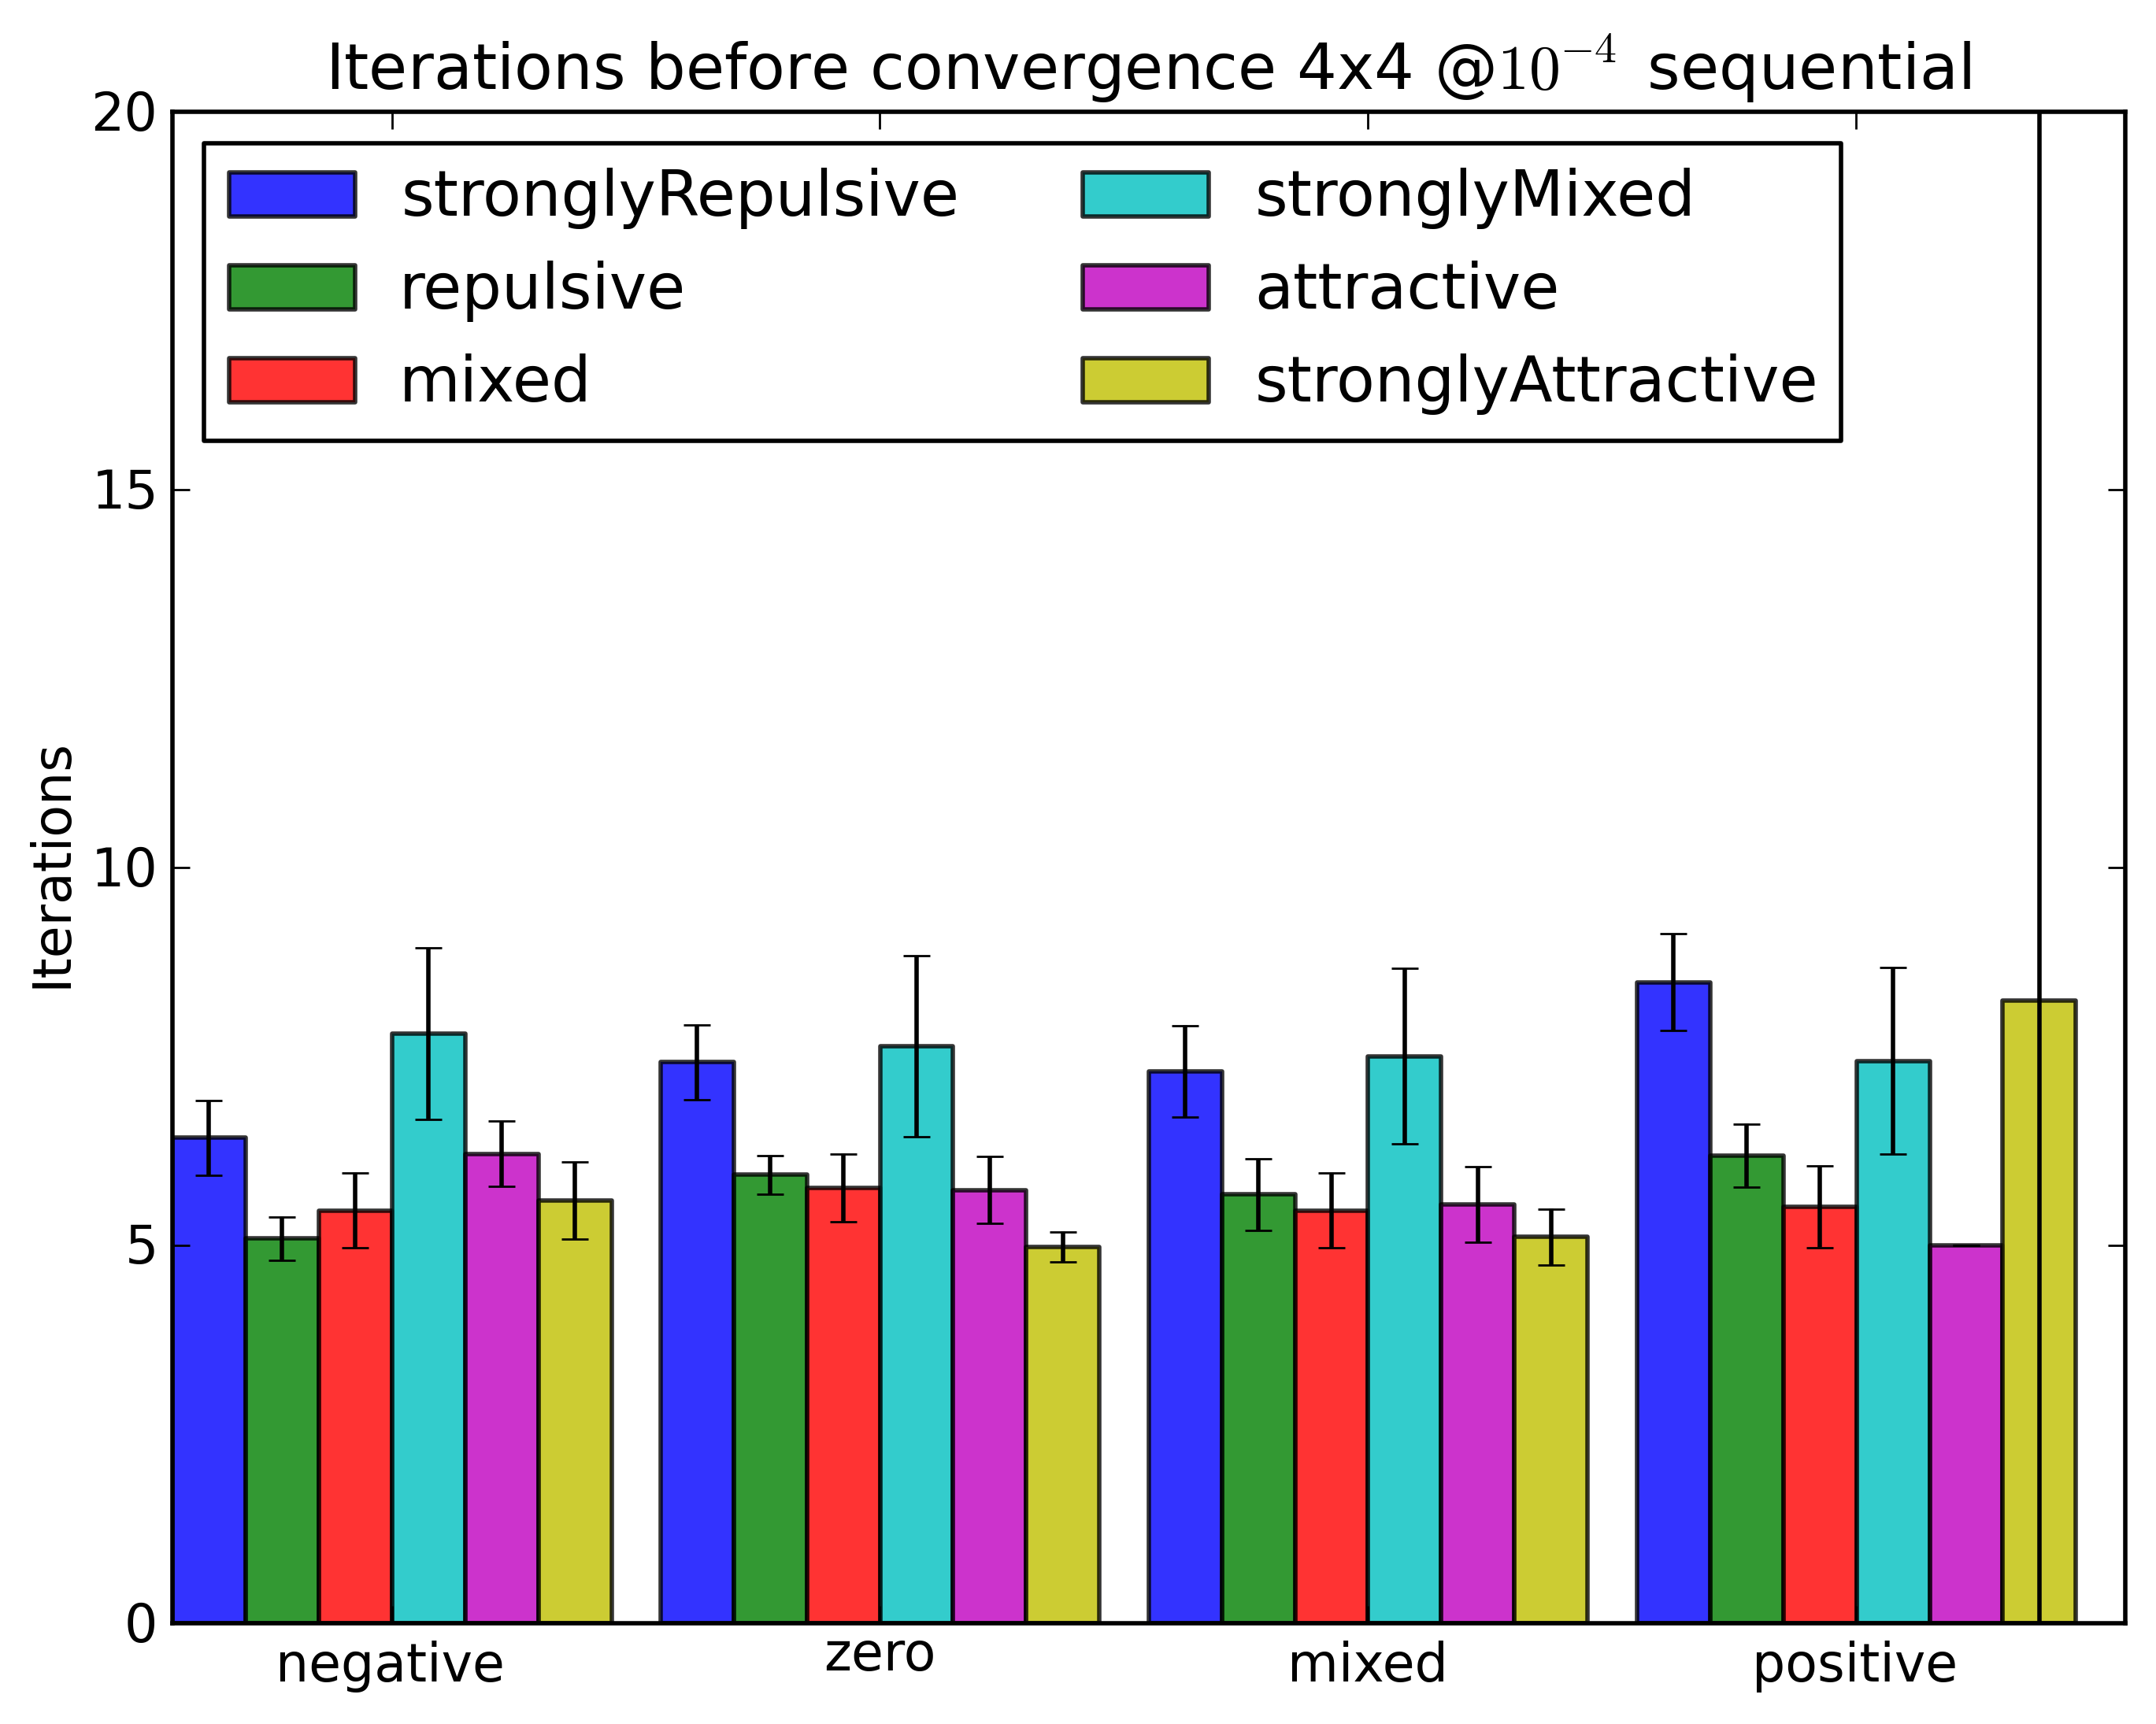
\includegraphics[width=6.5cm]{plots/convergence/iterations_before_convergence_4x4_e-4_sequential.png}}
  \subfigure[Naive parallel EP]{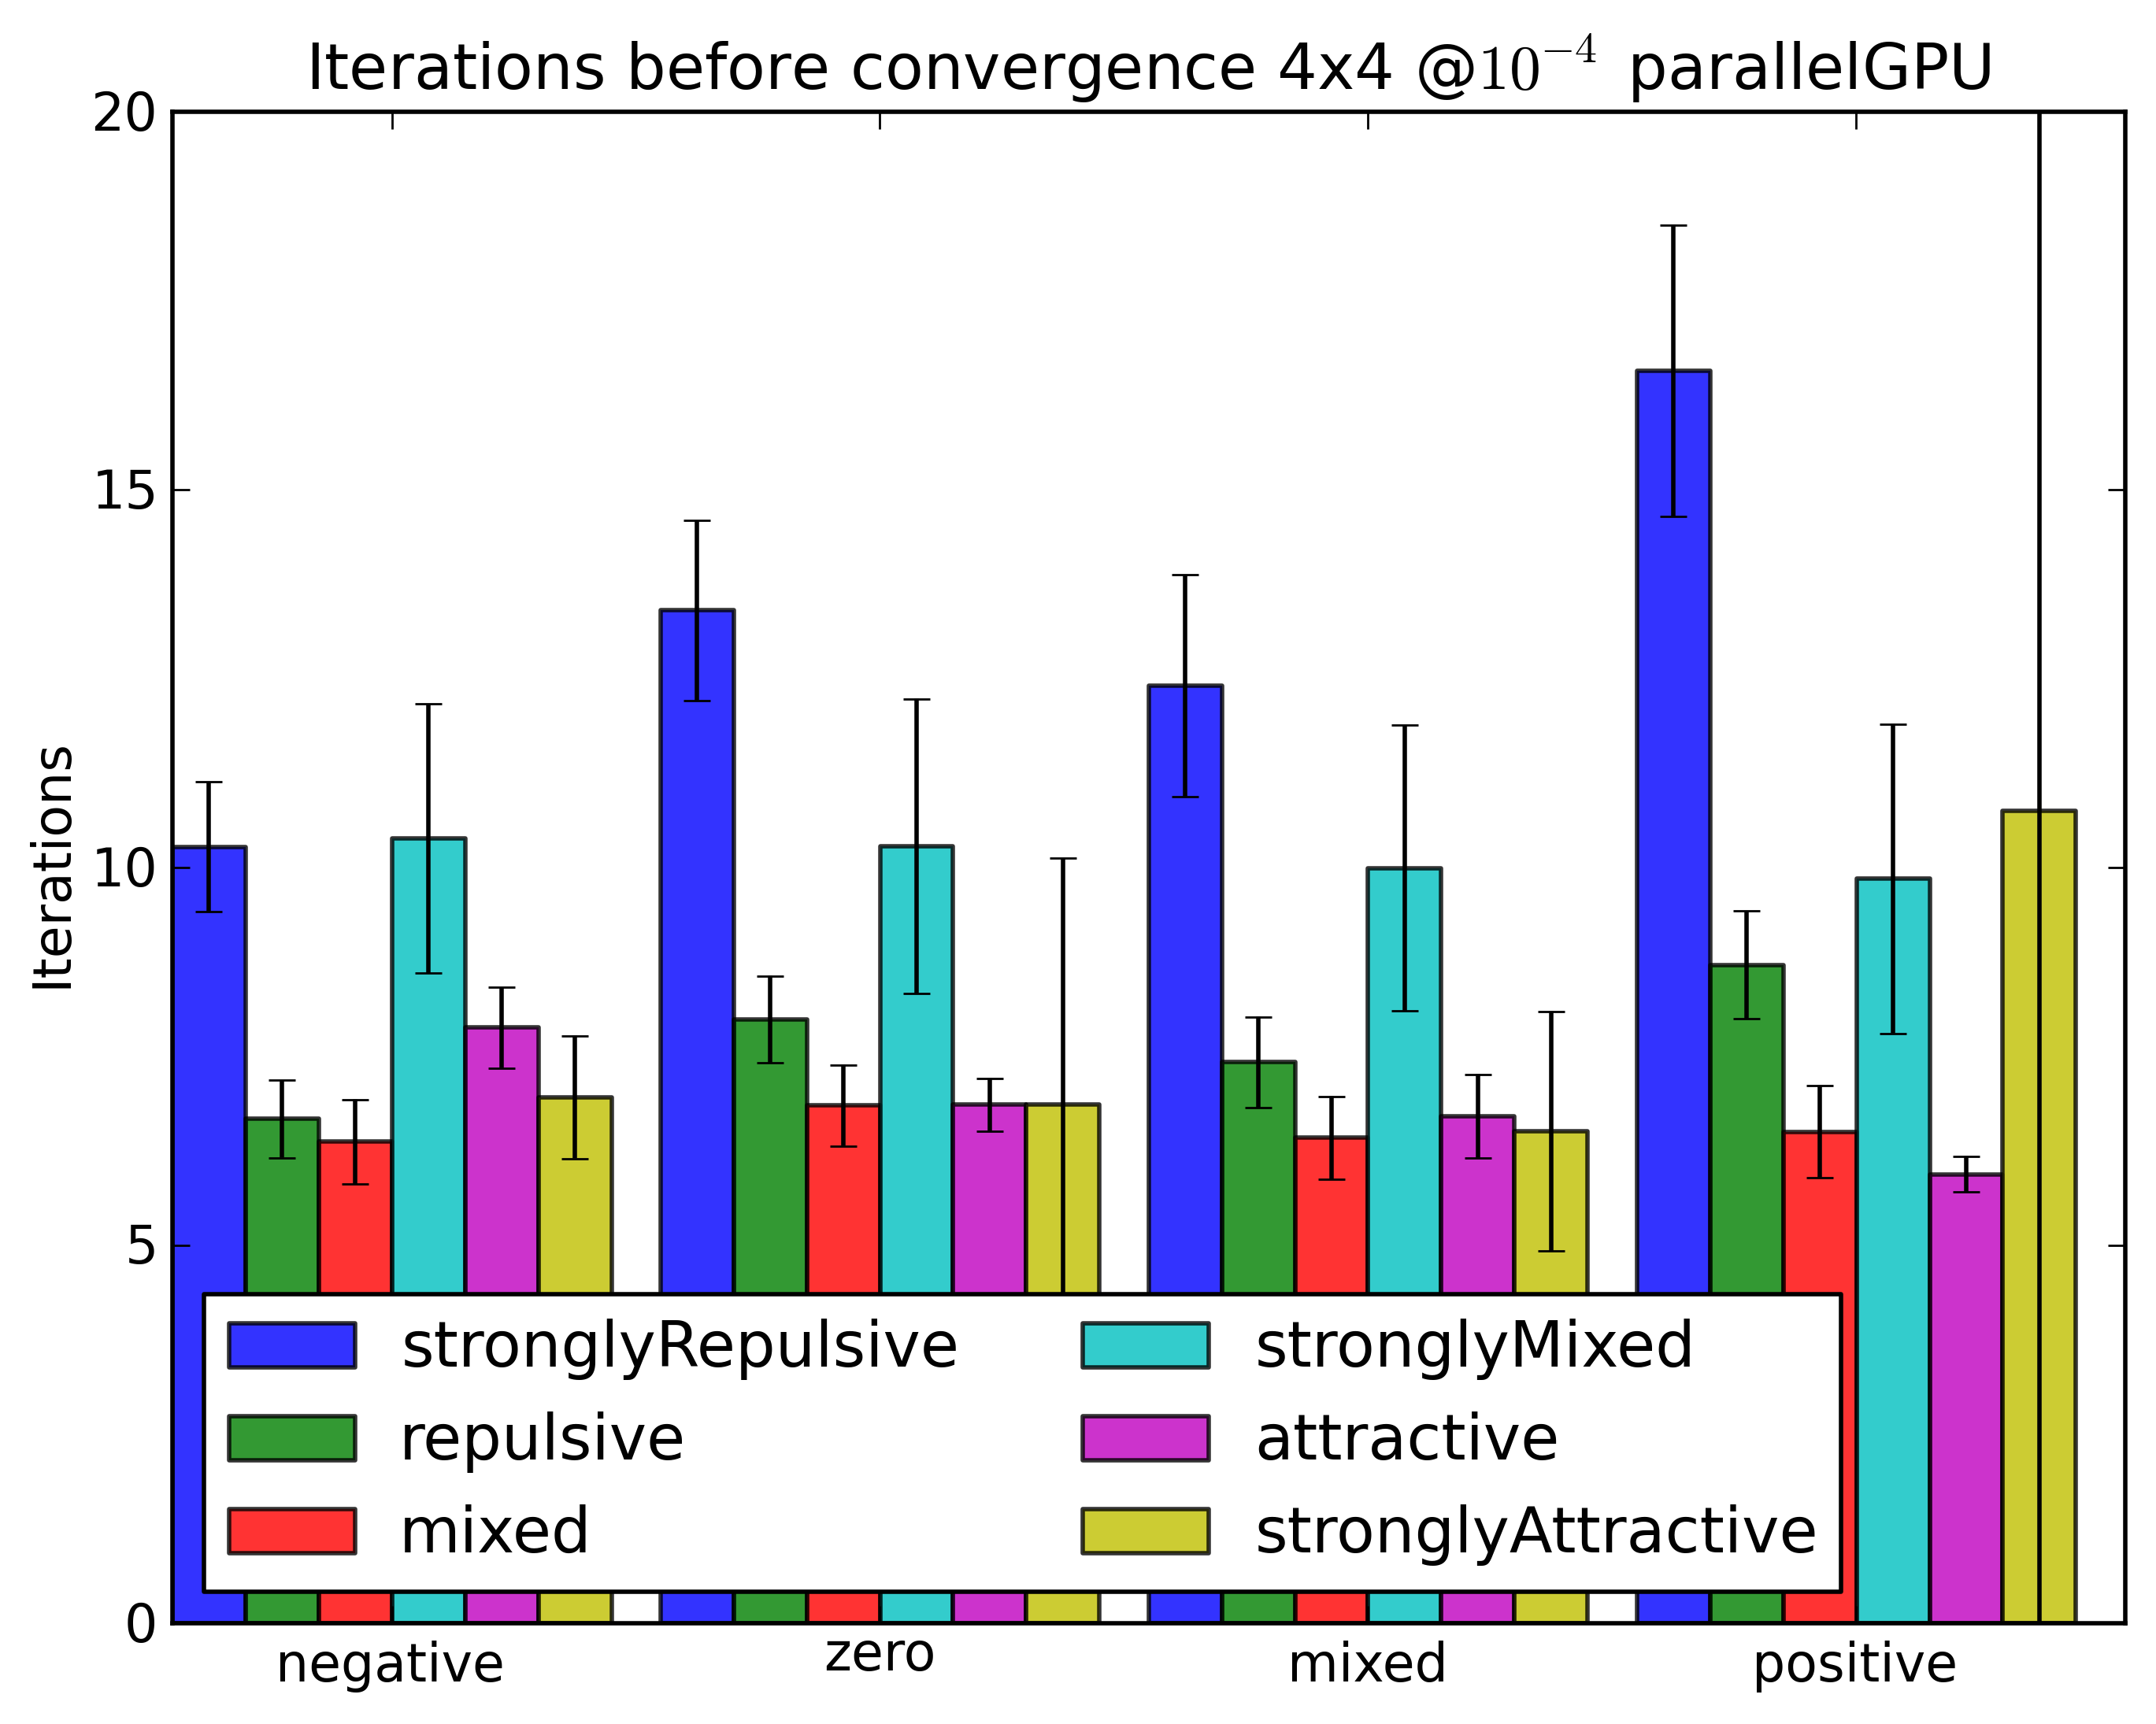
\includegraphics[width=6.5cm]{plots/convergence/iterations_before_convergence_4x4_e-4_parallelGPU.png}} 
	\subfigure[Convexified EP]{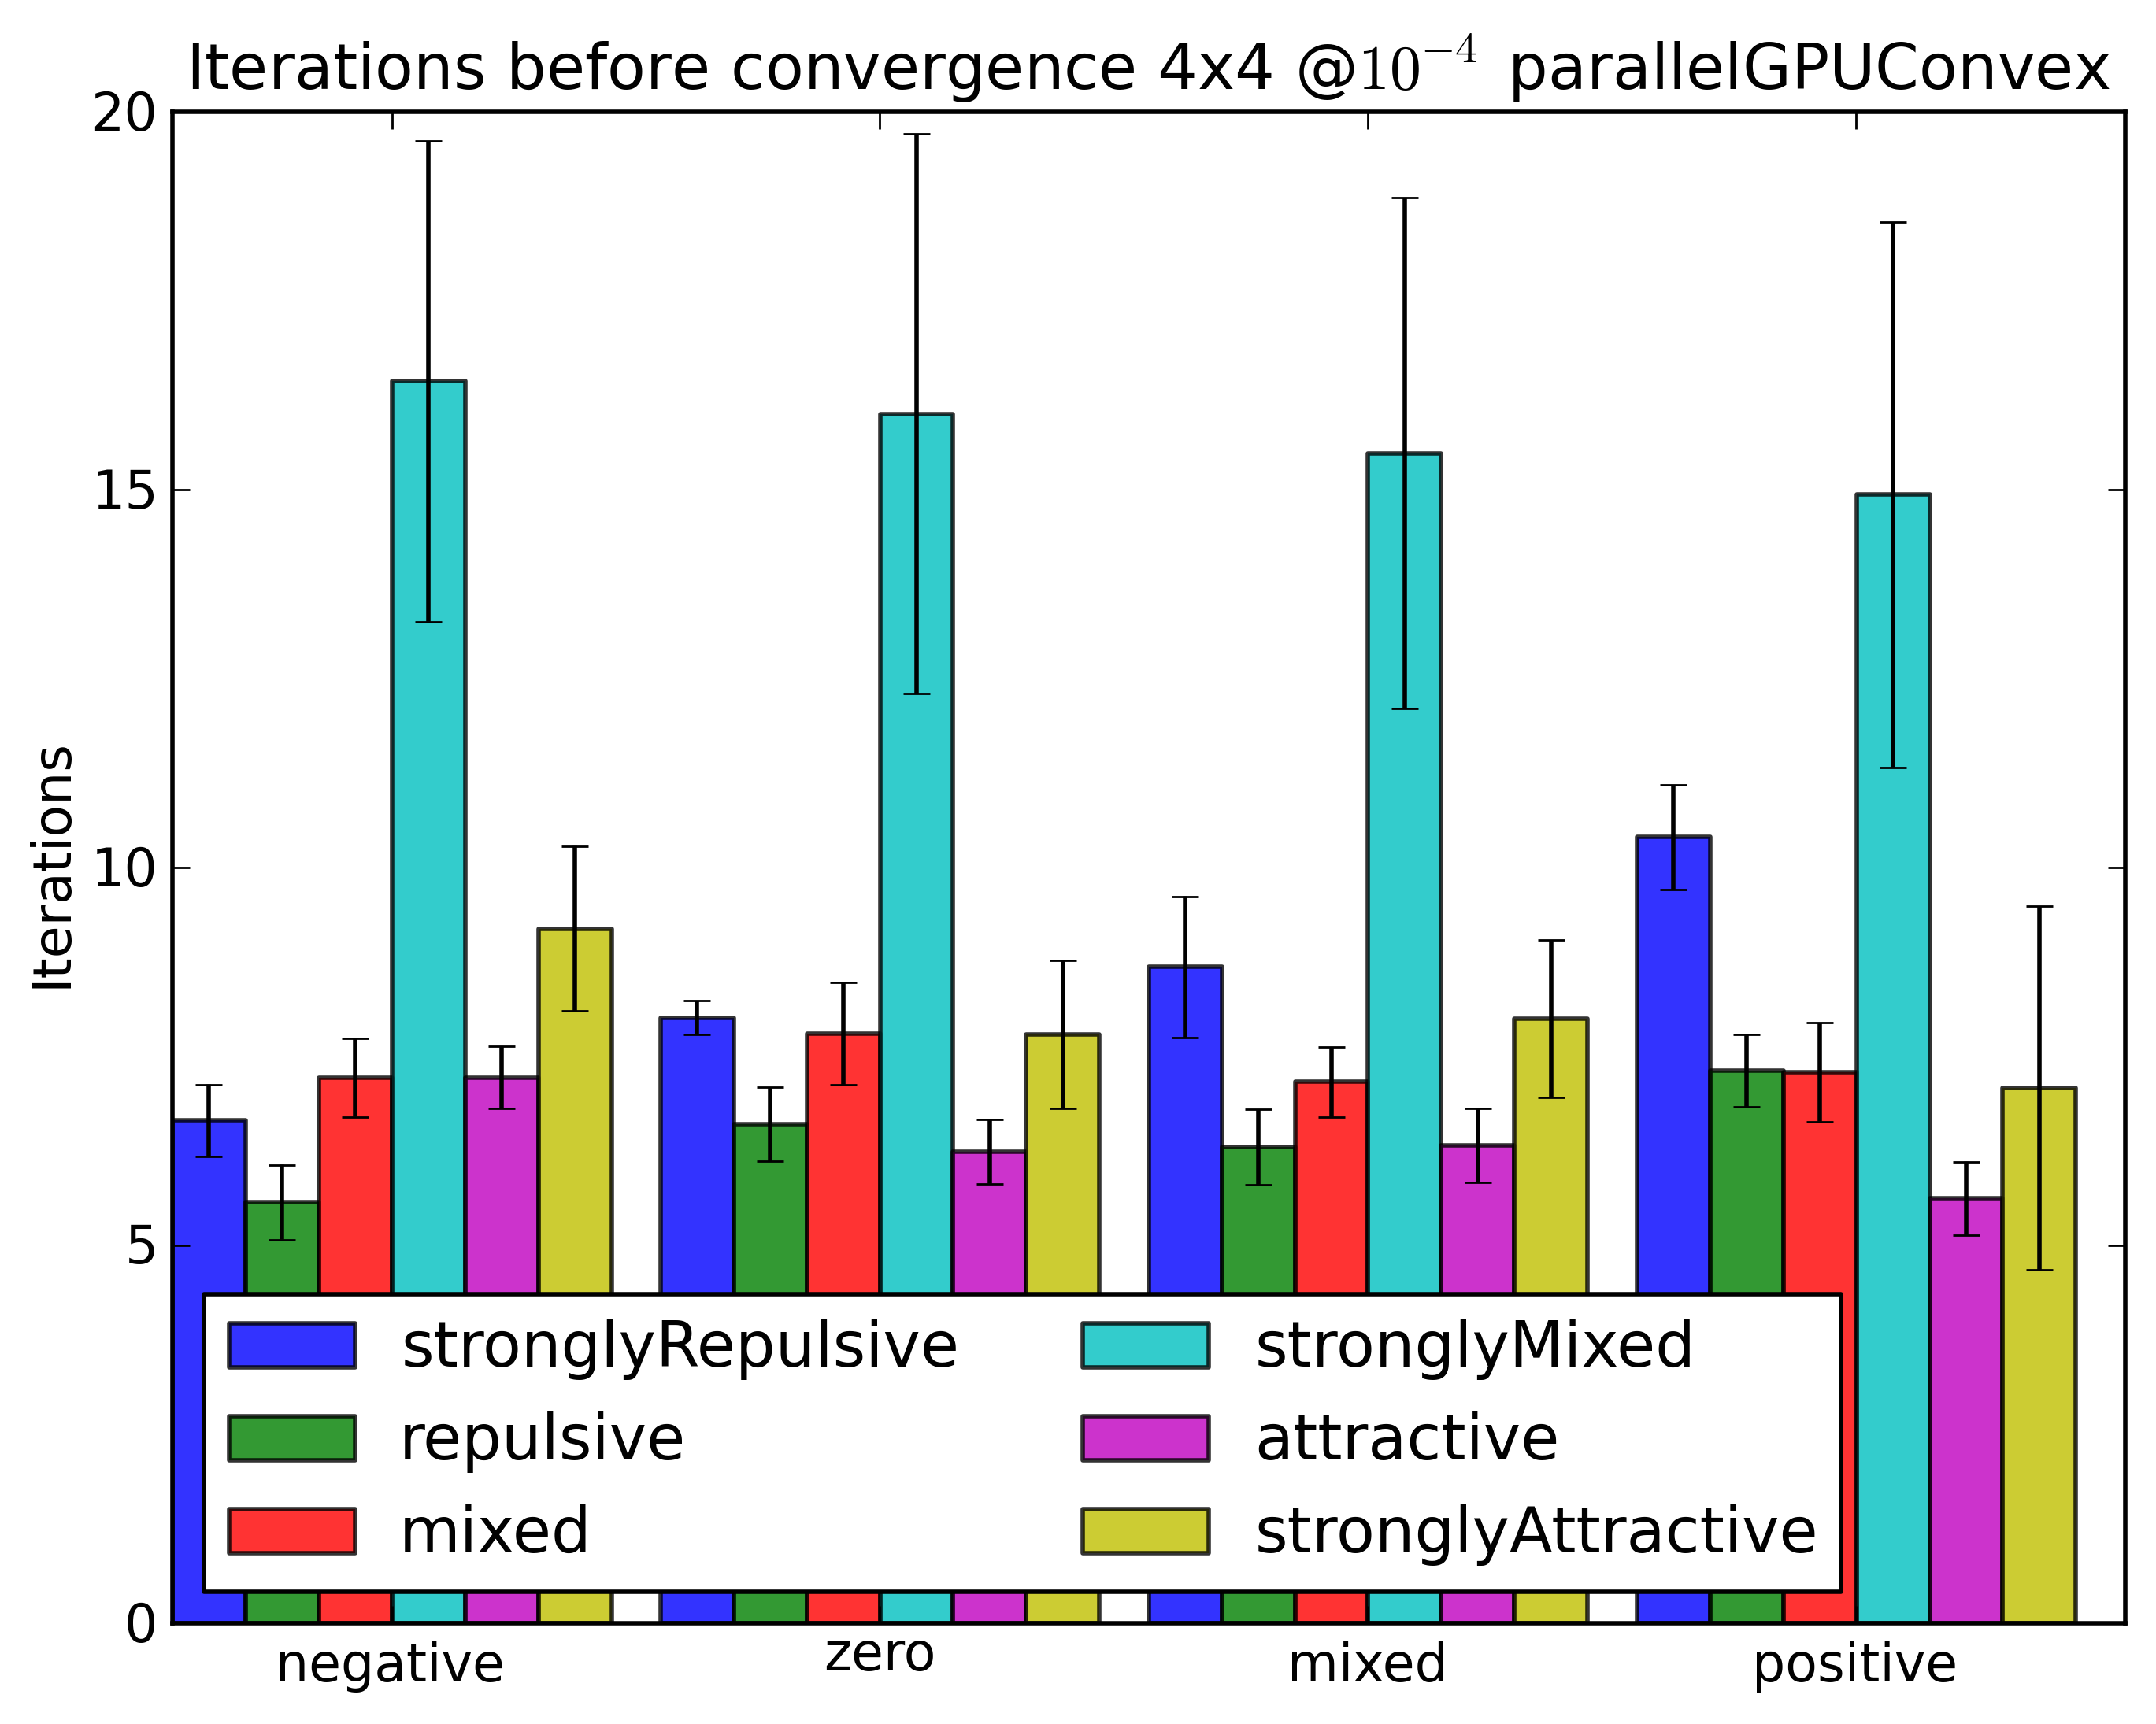
\includegraphics[width=6.5cm]{plots/convergence/iterations_before_convergence_4x4_e-4_parallelGPUConvex.png}}
  \subfigure[Pseudo-Convexified EP]{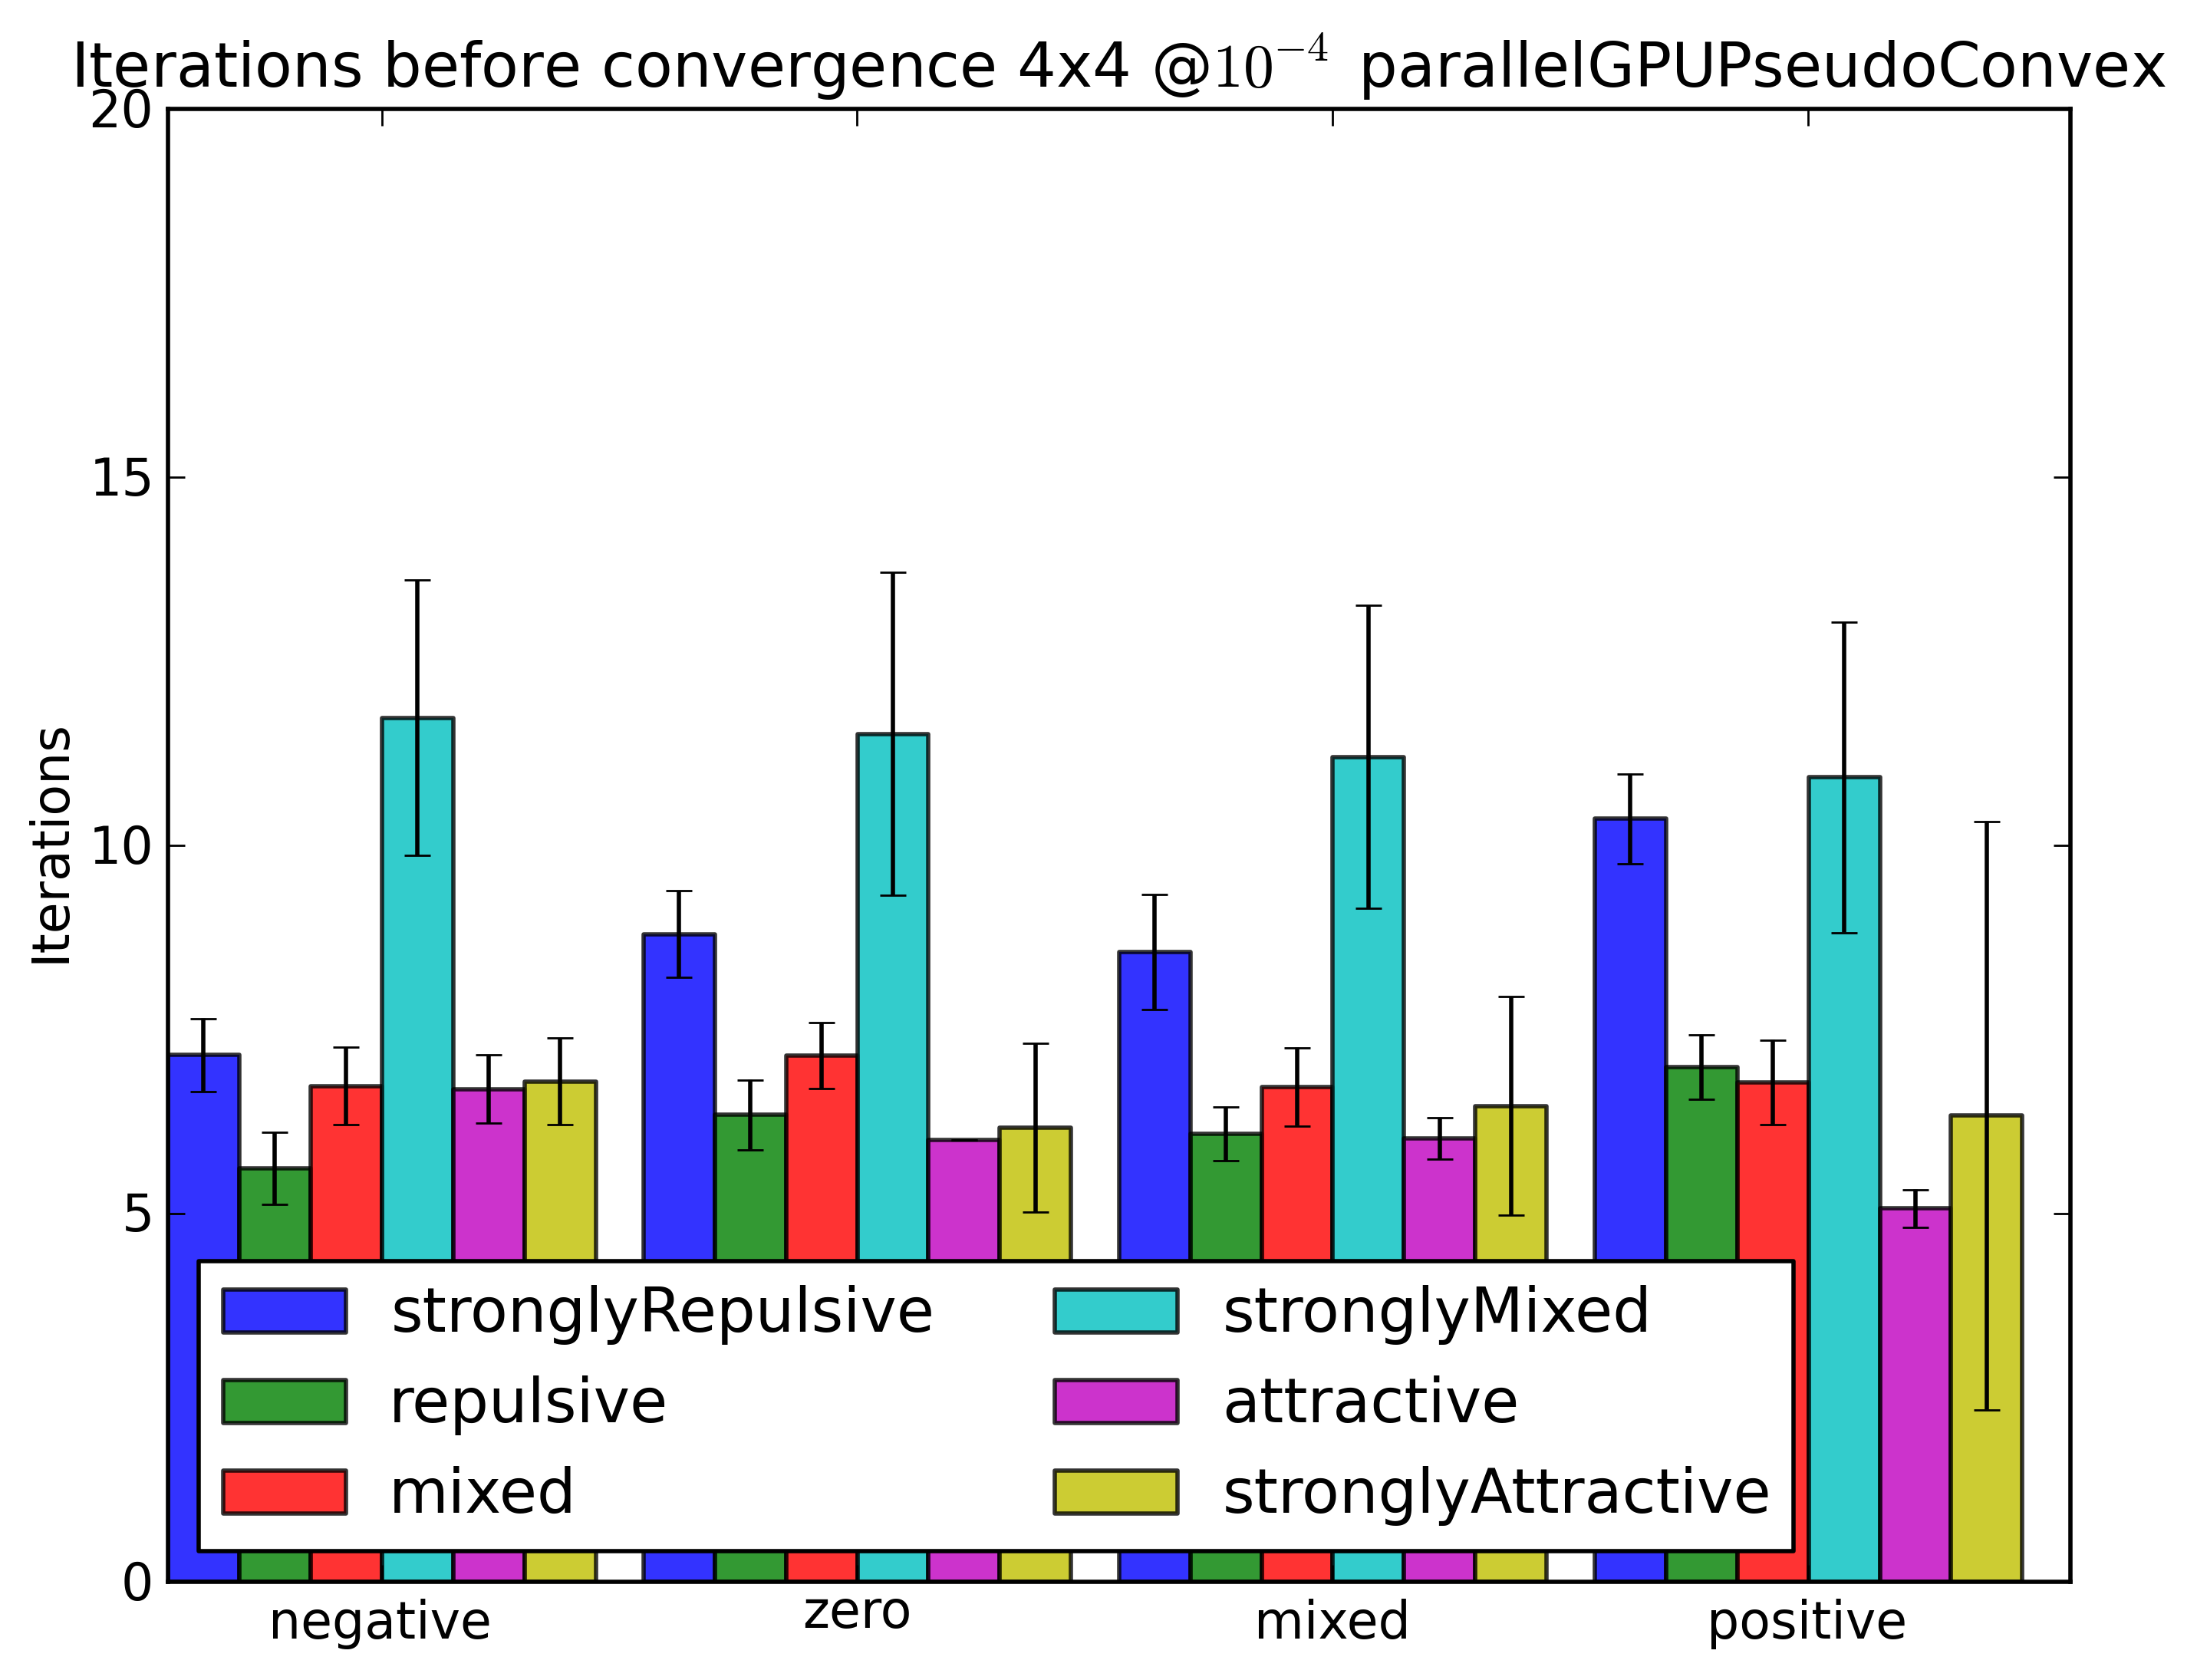
\includegraphics[width=6.5cm]{plots/convergence/iterations_before_convergence_4x4_e-4_parallelGPUPseudoConvex.png}}
	\caption{Number of iterations before computed marginals change less than $10^{-4}$ in relative $L_1$ norm. Results are averaged over 100 $4 \times 4$ Ising instances per Ising type. Error bars are shown at 1 sigma.}
	\label{44conv}
\end{figure}
\section{Evaluation}
We now turn to a practical evaluation of the derived robustified EP. We chose to evaluate the robustified EP on Ising model instances because of the model universality, ease of parametrization and relatively straightforward implementation for the GPU. We start by a short introduction to the Ising model and give an operational definition of the inference task we are solving. After rapidly going through the actual implementation, we present a complete set of measurements which describe the algorithm performance with respect to convergence, accuracy and speed.

\subsection{Ising model}
The two dimensional Ising model is defined by the quartet $(n, m, (\theta_i)_i, (\theta_{i,j})_{i,j})$ where $n, m \in \mathbb{N}$ represent the number of rows and columns of the model grid, $\theta_. \in \mathbb{R}^{nm}$ define the singleton potentials and $\theta_{.,.} \in \mathbb{R}^{2nm-n-m}$ the pair potentials. For 0/1 valued variables, the corresponding joint probability writes:
\[
	p(x_1,\dots,x_{nm}) \propto \prod_i e^{\theta_i x_i} \prod_{i,j} e^{\theta_{i,j} (x_i x_j + (1-x_i)(1-x_j))}
\]
which we usually express in the log domain:
\[
	p \propto \sum_i \theta_i x_i + \sum_{i,j} \theta_{i,j} (x_i x_j
  + (1-x_i)(1-x_j)) + \mathrm{const}
\]

There are mainly two inference tasks one is interested in. The
obvious one is determining the mode of $\log p$, e.g. the
configuration of $x$ variables which maximize the probability. A
second one is computing the $nm$ marginals $p(x_i)$. This is
precisely what EP as previously defined achieves. In particular,
the goal is to approximate $p$ by a simpler distribution $q$ where each variable is decoupled. 
\[
\log q = \sum_i \tilde \theta_i x_i + \mathrm{const}
\]
It is clear that computing the $\tilde \theta$ parameters directly yields the marginals we want, by namely $p(x_i) \approx \frac{1}{1+e^{-\tilde \theta_i}}$. Thus, to evaluate our algorithm, we compute the $\tilde \theta$ parameters exactly by explicit marginalization when possible (in practice, the problem becomes intractable for sizes larger than $5 \times 6$ with our naive exact implementation), and approximately using our algorithm.

Ising models exhibit a rich behavior which depends on how the different parameters are chosen. Table \ref{typo} defines the typology of Ising models we use in the evaluation.

\begin{table}[!h]\centering
	\subtable{
	\begin{tabular}{c|c}
		Name & $\theta_i$ \\
		\hline
		negative & $ \unif[-1; 0]$ \\
		zero & $0$\\
		mixed & $ \unif[-1;1]$\\
		positive & $ \unif[0;1]$\\
	\end{tabular}}\subtable{
	\begin{tabular}{c|c}
		Name & $\theta_{i,j}$ \\
		\hline
		strongly repulsive & $ \unif[-3; 0]$ \\
		repulsive & $\unif[-1;0]$\\
		mixed & $ \unif[-1;1]$\\
		strongly mixed & $ \unif[-3;3]$\\
		attractive & $ \unif[0;1]$\\
		strongly attractive & $ \unif[0;3]$\\
	\end{tabular}}
	\caption{Singleton and pair potential typology. $\unif$ is the uniform distribution.}
	\label{typo}
\end{table}



\subsection{Implementation}
We have implemented an exact marginalization code, a vanilla
sequential EP and an OpenCL parallel version of EP. As the
difference between the naive parallelization of EP and the
convexified parallelization of EP is only a parameter (the power
exponent $\frac1\rho$), there is no separate implementation for the robustified EP. In what follows, we call \emph{convex EP} a parallel EP with $\rho=2$, and \emph{pseudo-convex EP} a parallel EP with $\rho=1.5$. For all of the implementations, we ran into underflow issues which were successfully solved by performing all the computations in the log domain, namely, we only work with log values. This is not a problem where the original algorithm contains multiplication and exponentiation, but requires an log-exp operation and a conditional\footnote{$\log(e^a+e^b)=a+\log(1+\exp(b-a))$ if $a>b$; $\log(e^a+e^b)=b+\log(1+\exp(a-b))$ else} whenever we add two log values. This significantly reduces performance.

Following OpenCL terminology, the heart of the parallel implementation is a kernel function (75 lines of C code) which is executed by the workers of the OpenCL target device. The parallelization is such that each worker is identified to an edge of the model. Two in device-memory tables contain the computed messages (one for the messages of the previous iteration, one for the current messages being computed) and the corresponding input pointers are swapped between each iteration. In sum, each worker updates its portion of the messages table, and a corresponding one full sequential iteration of EP is achieved when all the workers on the edges finished their updates. The only conditionals the kernel contains are these introduced by the previously mentioned log add operation.

In effect, the OpenCL implementation is quite concise if one ignores the overhead of the setup code (specifying the device, creating the command queues, compiling the kernel for the device, adjusting parameters, moving data around, \dots).

As for any optimization algorithm, we are interested in evaluating three characteristics: convergence, defined as the number of iterations before the output changes by less than a given threshold; accuracy defined as the error between the approximate and the exact solution once convergence occurs; and last but not least speed.

\subsection{$4 \times 4$ models}
We start by determining challenging types of Ising models both in terms of convergence and accuracy for our algorithm. We use $4 \times 4$ Ising instances for a complete exploration of the space. Figure \ref{44conv} presents how convergence (if any) occurs on the $4 \times 6 = 24$ different types of Ising instances. Figure \ref{44acc} presents the corresponding results in terms of accuracy.


On $4 \times 4$ instances, instability rarely occurs. In effect, only positive strongly attractive instances result in an exploding number of iterations. As expected, the vanilla parallel EP usually results in longer convergence times. The convex EP does significantly reduce the convergence time in the strongly repulsive case and does converge in the positive strongly attractive case, but introduces more iterations on strongly mixed cases. The pseudo-convex EP has a beneficial effect on these but tends to increase instability for the positive strongly attractive case.

\begin{figure}[h!]\centering
	\subfigure[Sequential EP]{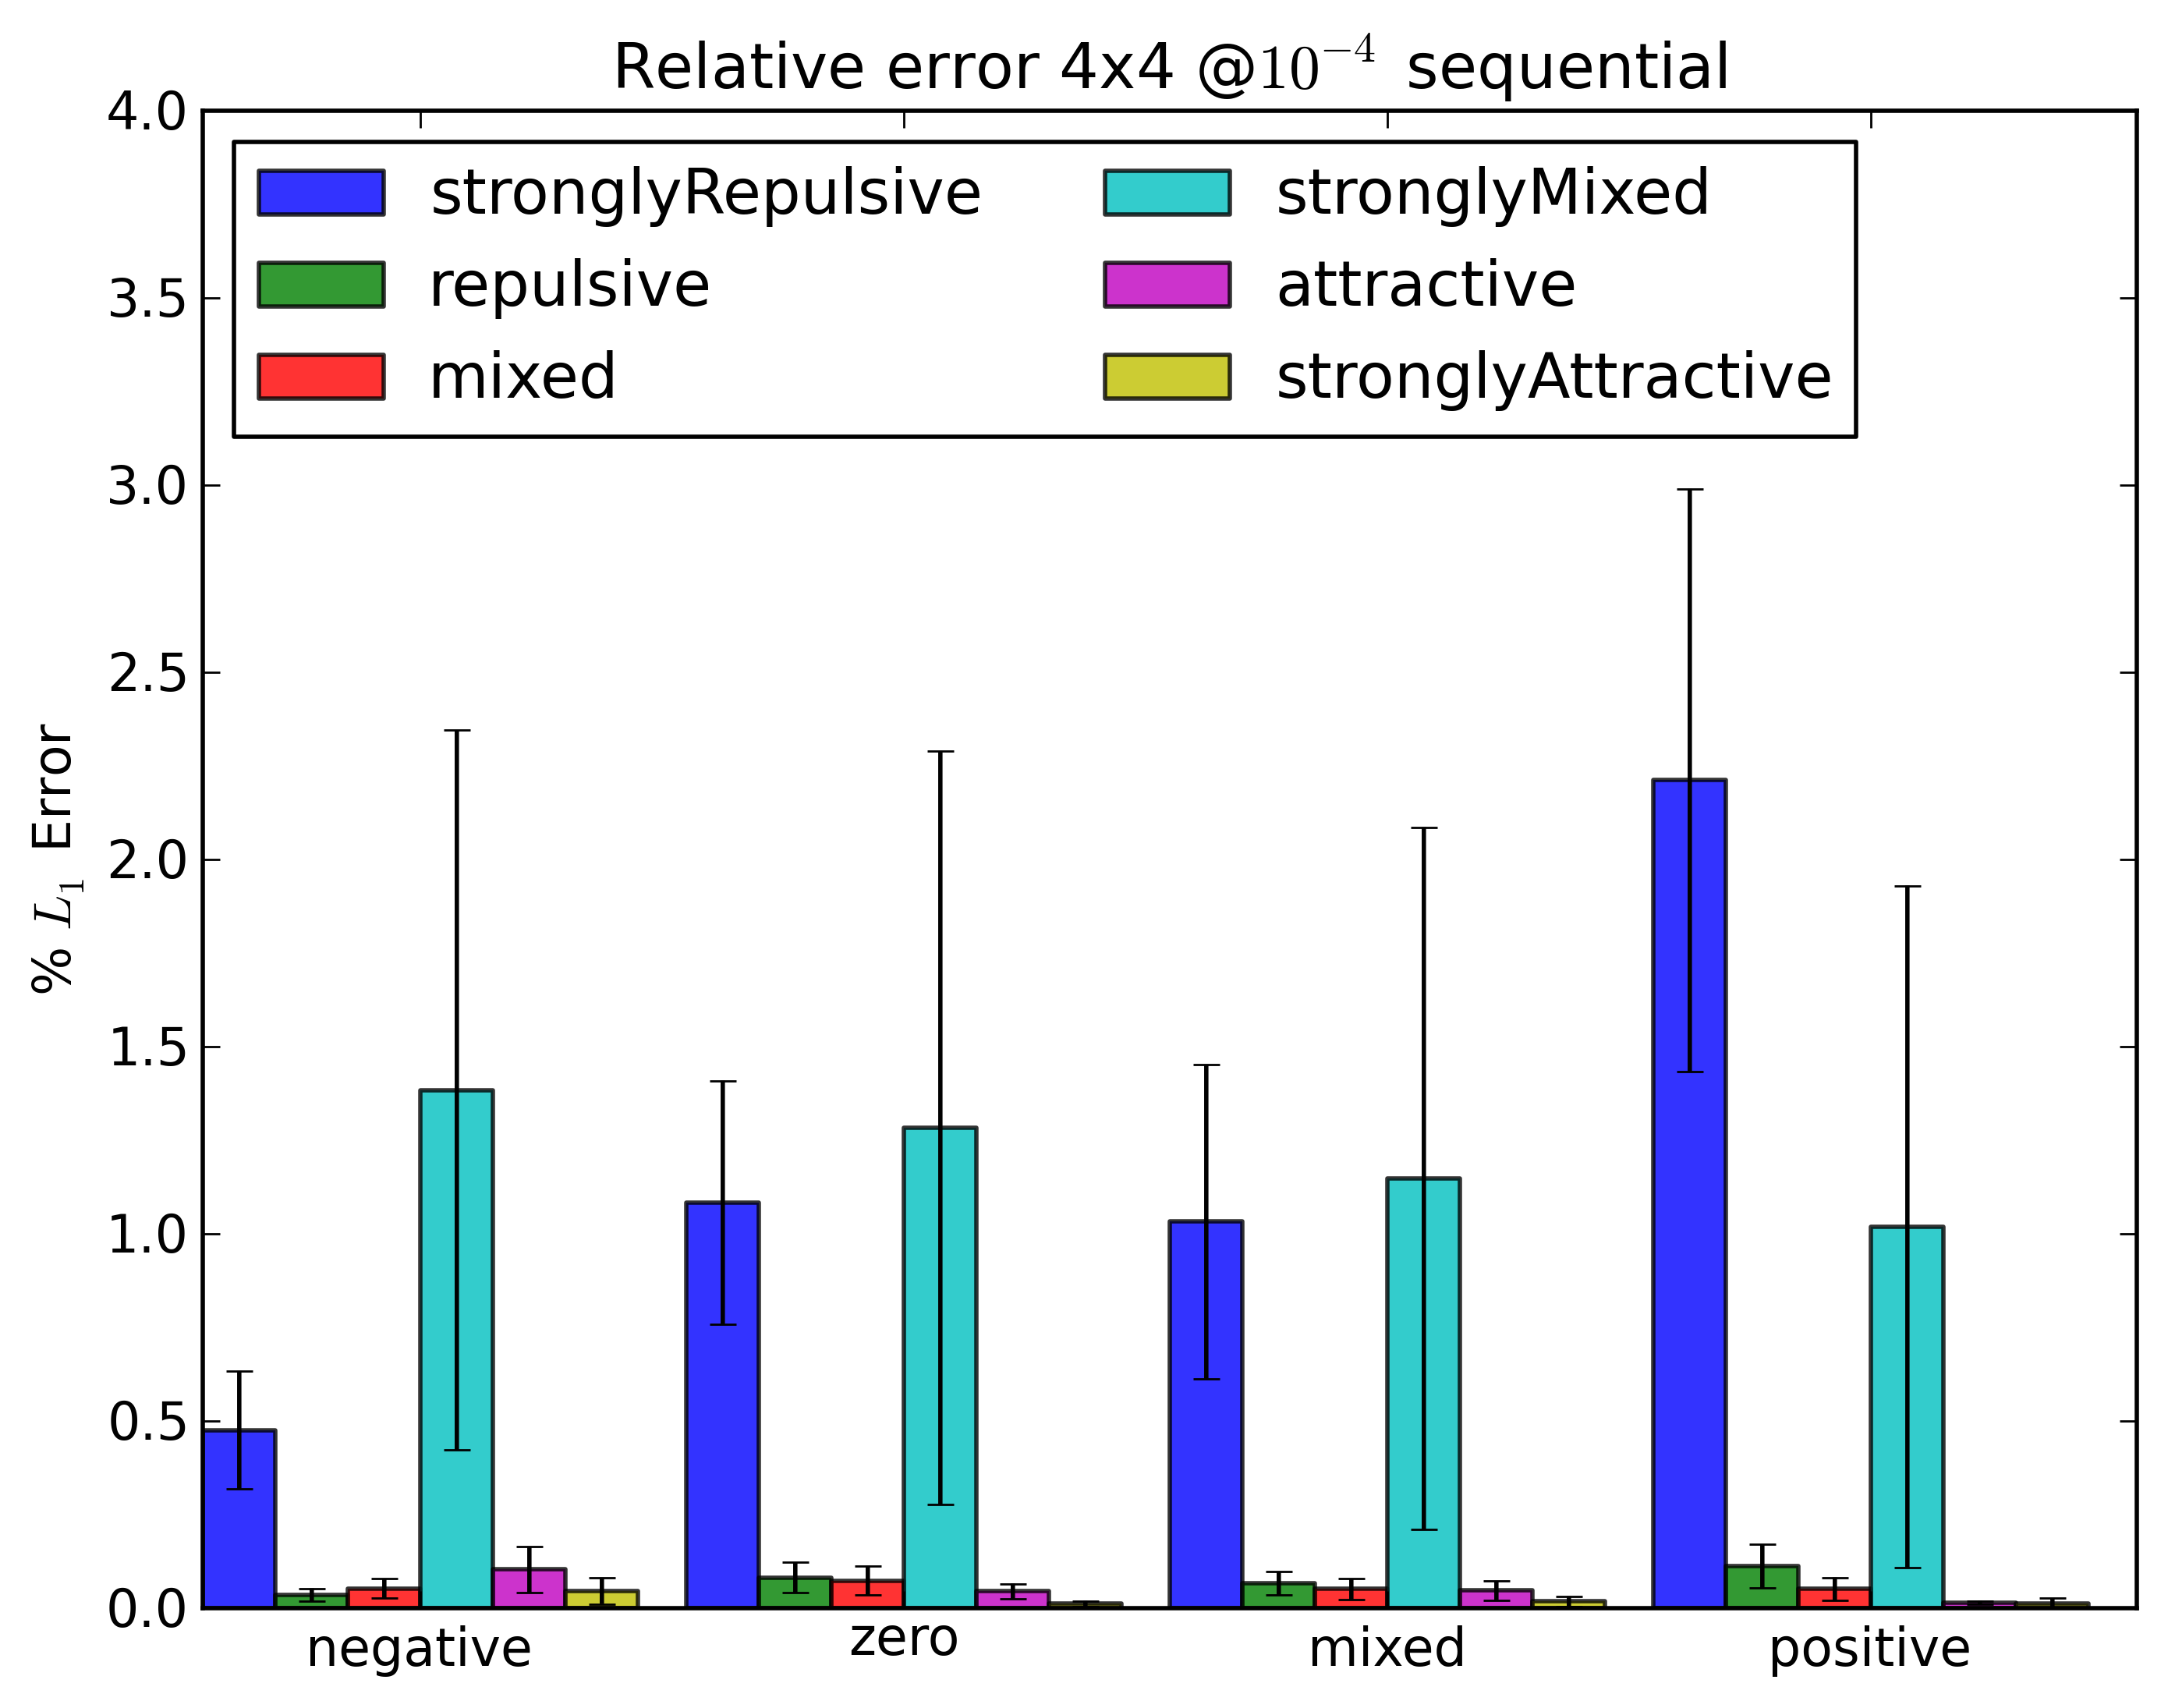
\includegraphics[width=6.5cm]{plots/accuracy/Relative_error_4x4_e-4_sequential.png}}
  \subfigure[Naive parallel EP]{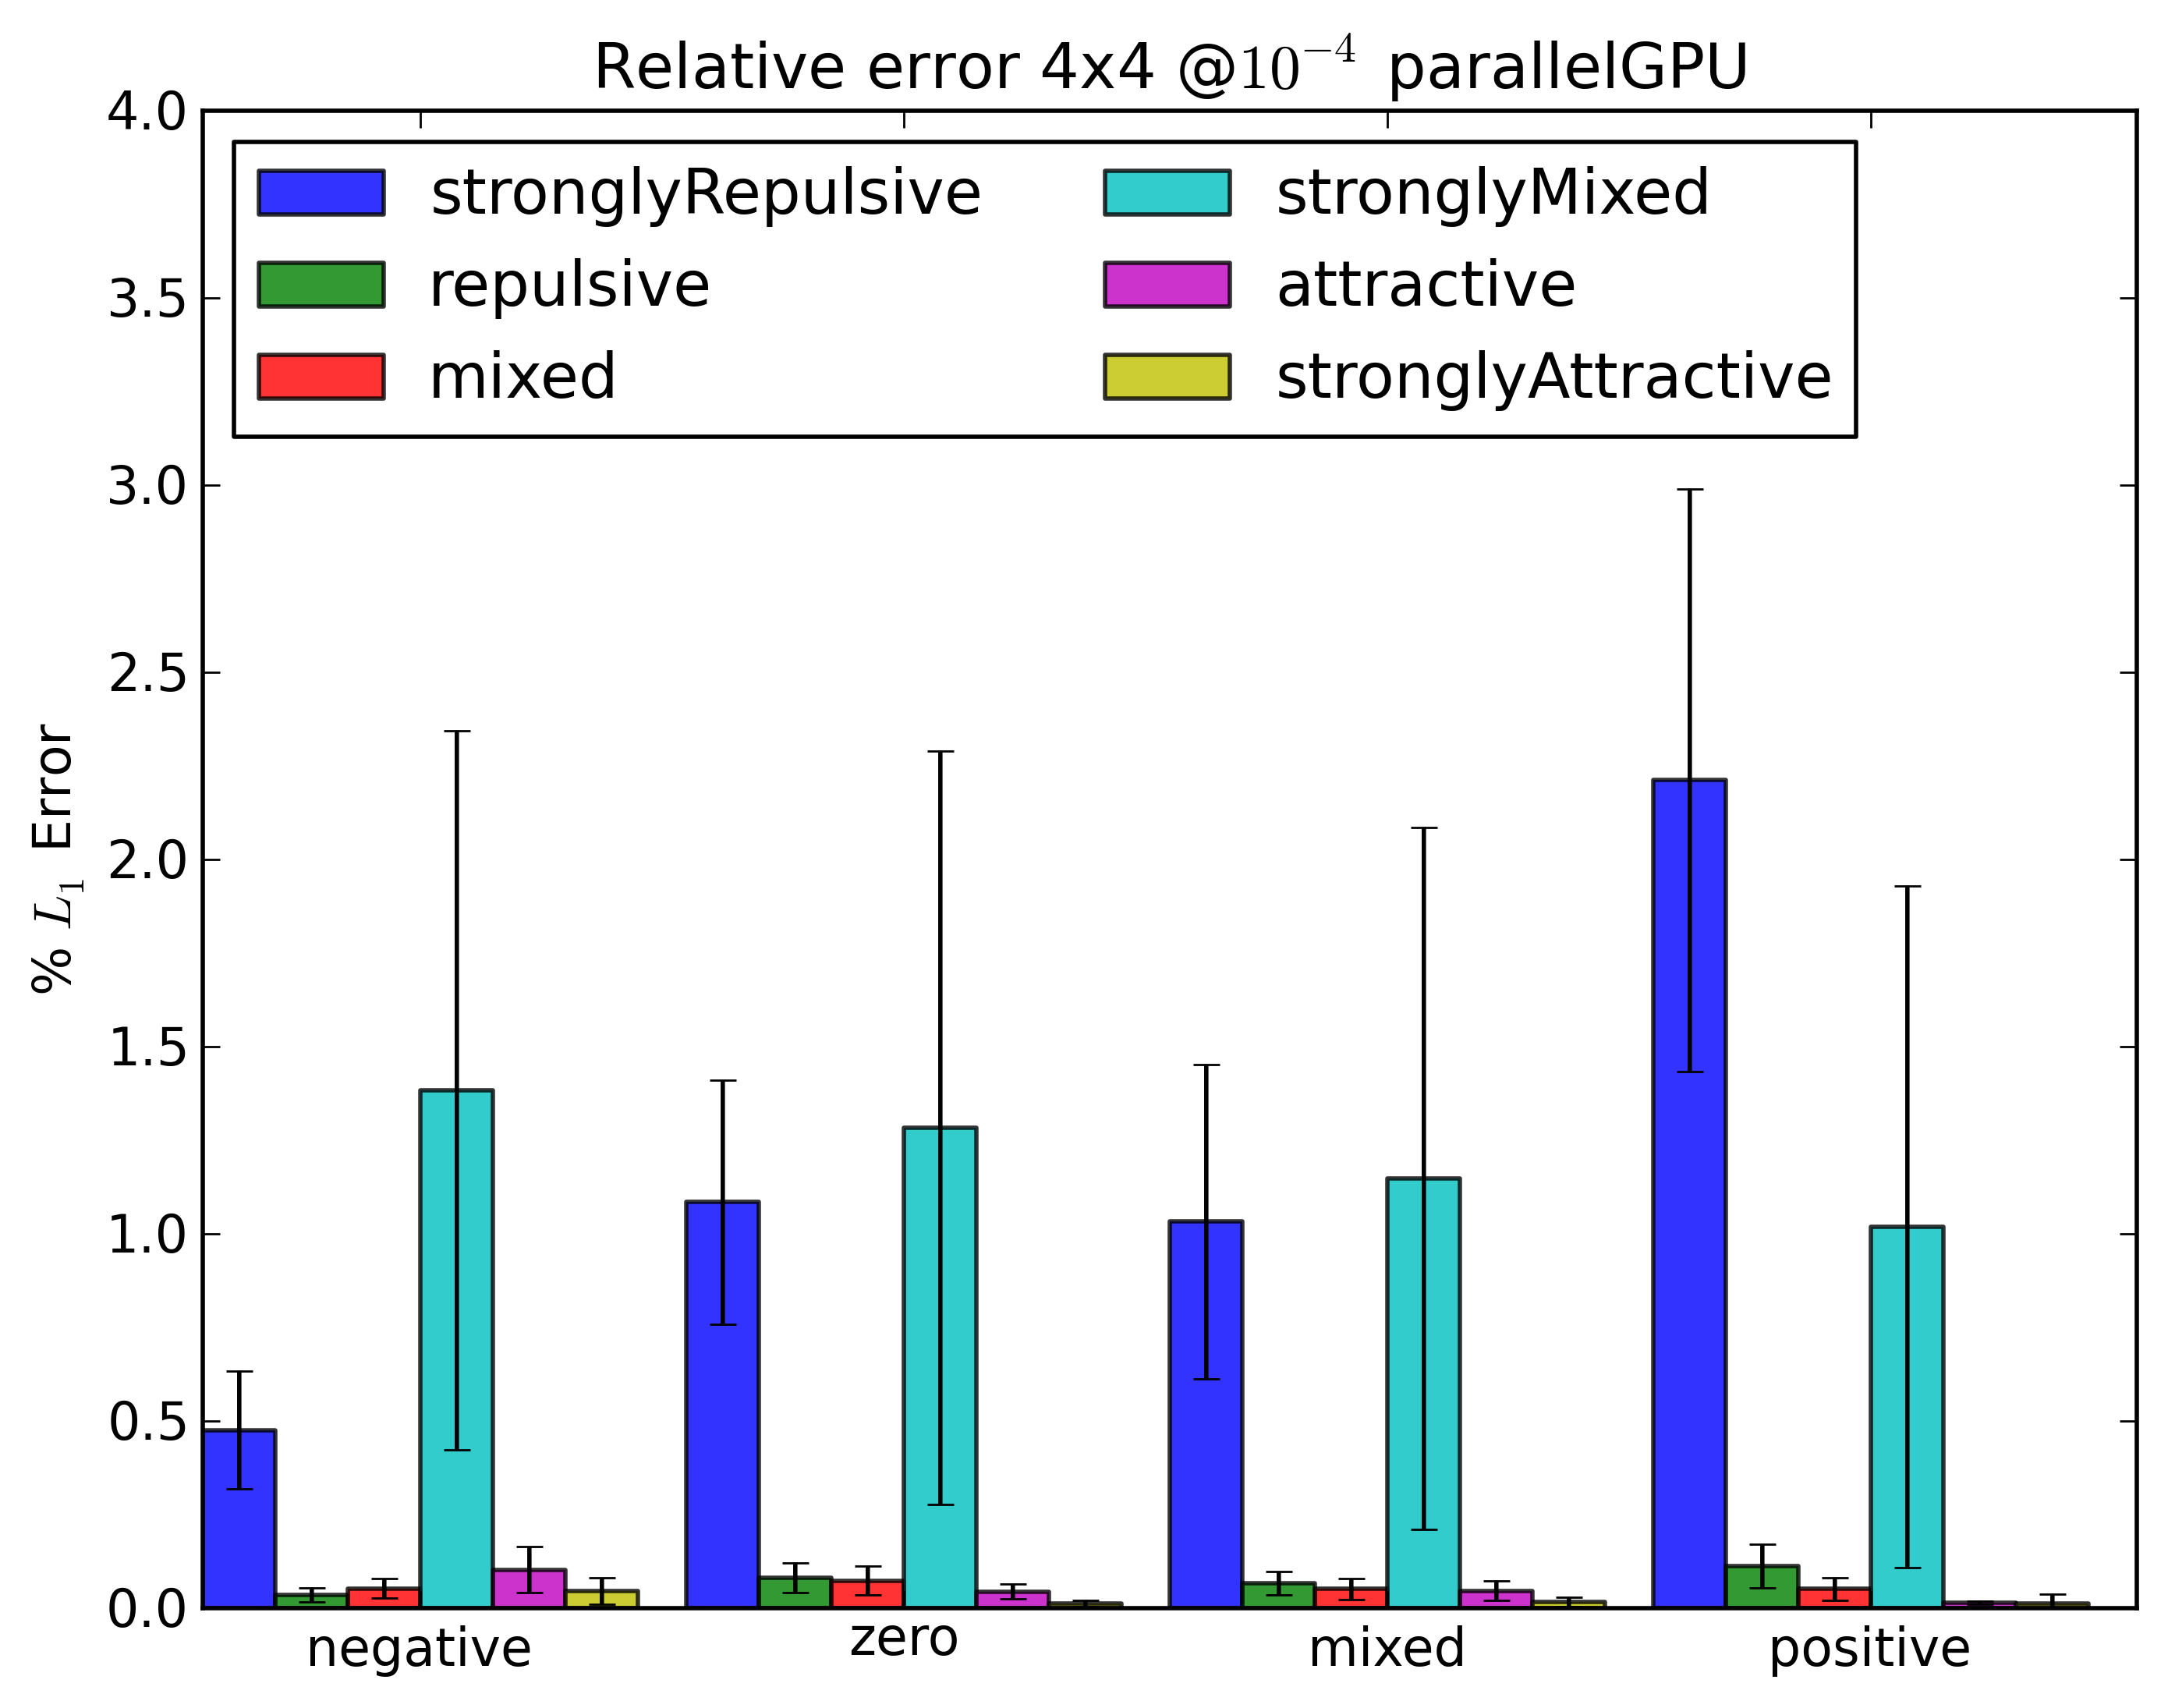
\includegraphics[width=6.5cm]{plots/accuracy/Relative_error_4x4_e-4_parallelGPU.png}}
	\subfigure[Convexified EP]{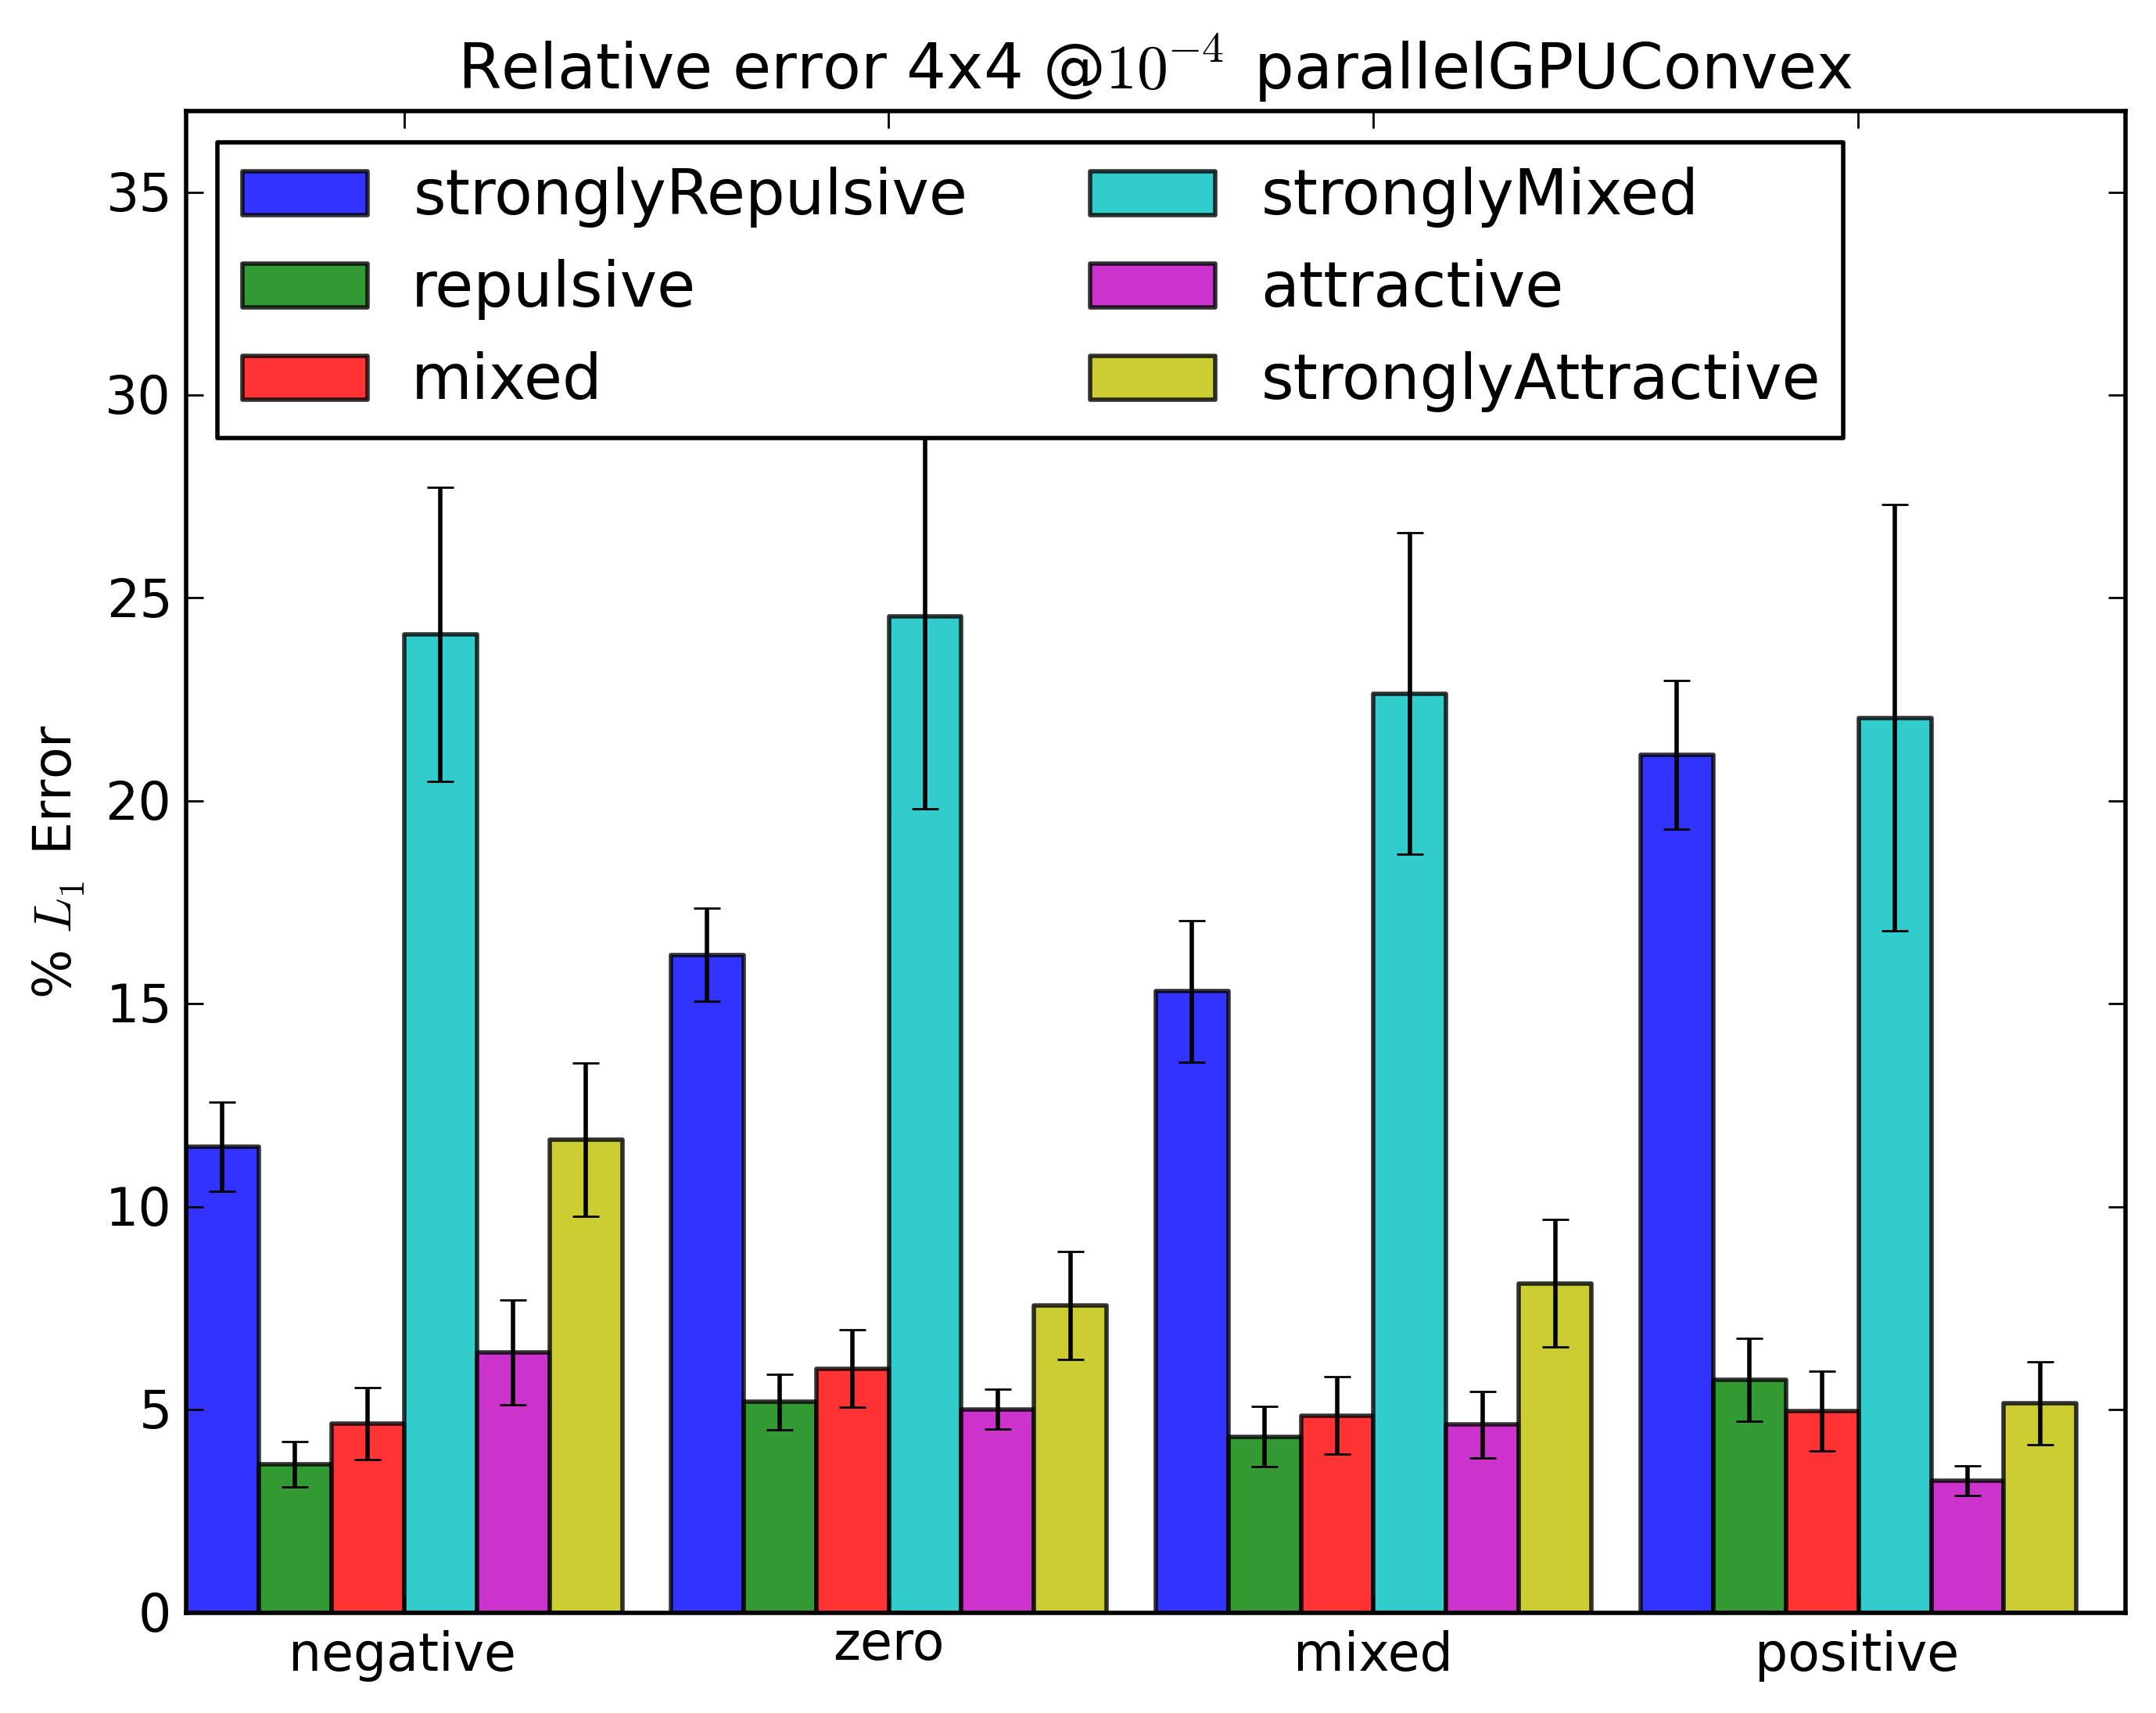
\includegraphics[width=6.5cm]{plots/accuracy/Relative_error_4x4_e-4_parallelGPUConvex.png}}
  \subfigure[Pseudo-Convexified EP]{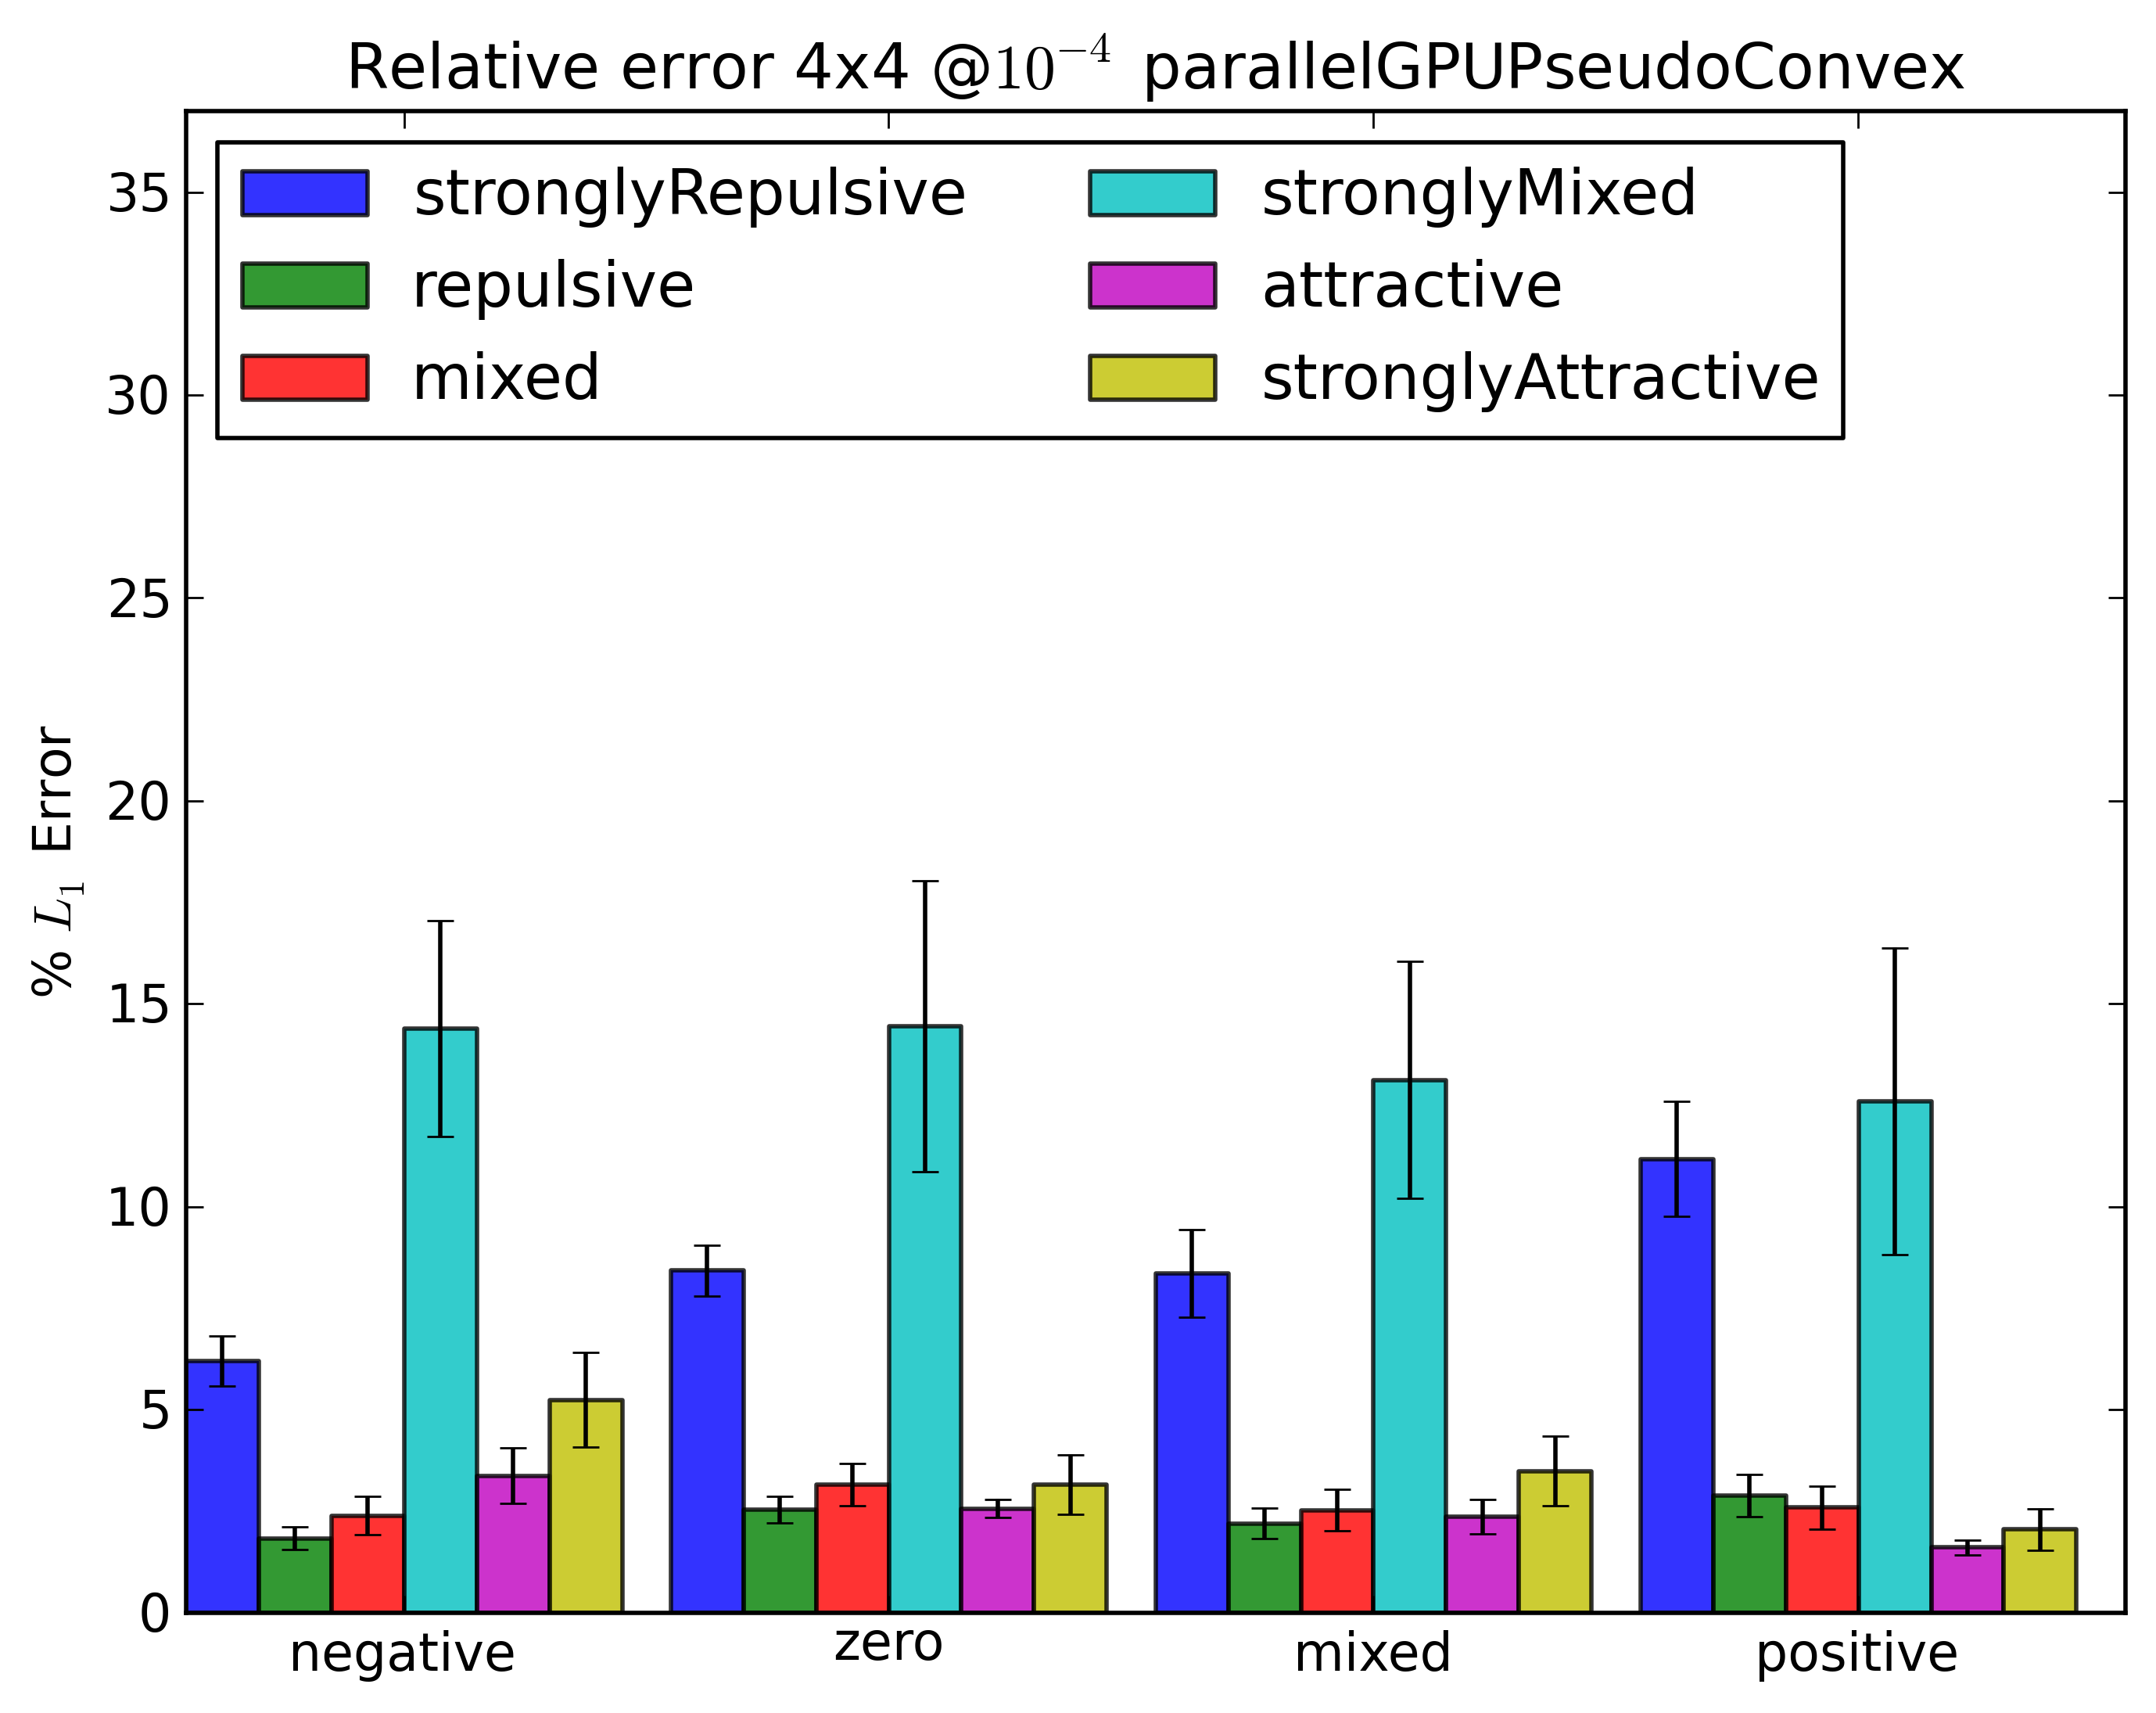
\includegraphics[width=6.5cm]{plots/accuracy/Relative_error_4x4_e-4_parallelGPUPseudoConvex.png}}
	\caption{Relative $L_1$ error after $10^{-4}$ convergence. Results are averaged over 100 $4 \times 4$ Ising instances per Ising type. Error bars are shown at 1 sigma.}
	\label{44acc}
\end{figure}

The price we pay for the improved convergence is depicted in figure \ref{44acc}. Both strongly repulsive and strongly mixed instances are generally hard for the algorithms. However, there is an order of magnitude more error for the convex EP when compared to the vanilla EP. Interestingly, there appears to be no significant accuracy difference between the sequential EP and the naive parallel EP. Finally, we can observe that pseudo-convex EP has a significantly better accuracy than convex EP.

Based on this exploration of the convergence-accuracy space, we want to focus on three interesting Ising instances: negative strongly mixed, positive strongly repulsive and positive strongly repulsive.

\subsection{Increasing model size}
\begin{figure}[ht!]\centering
	\subfigure[Convergence]{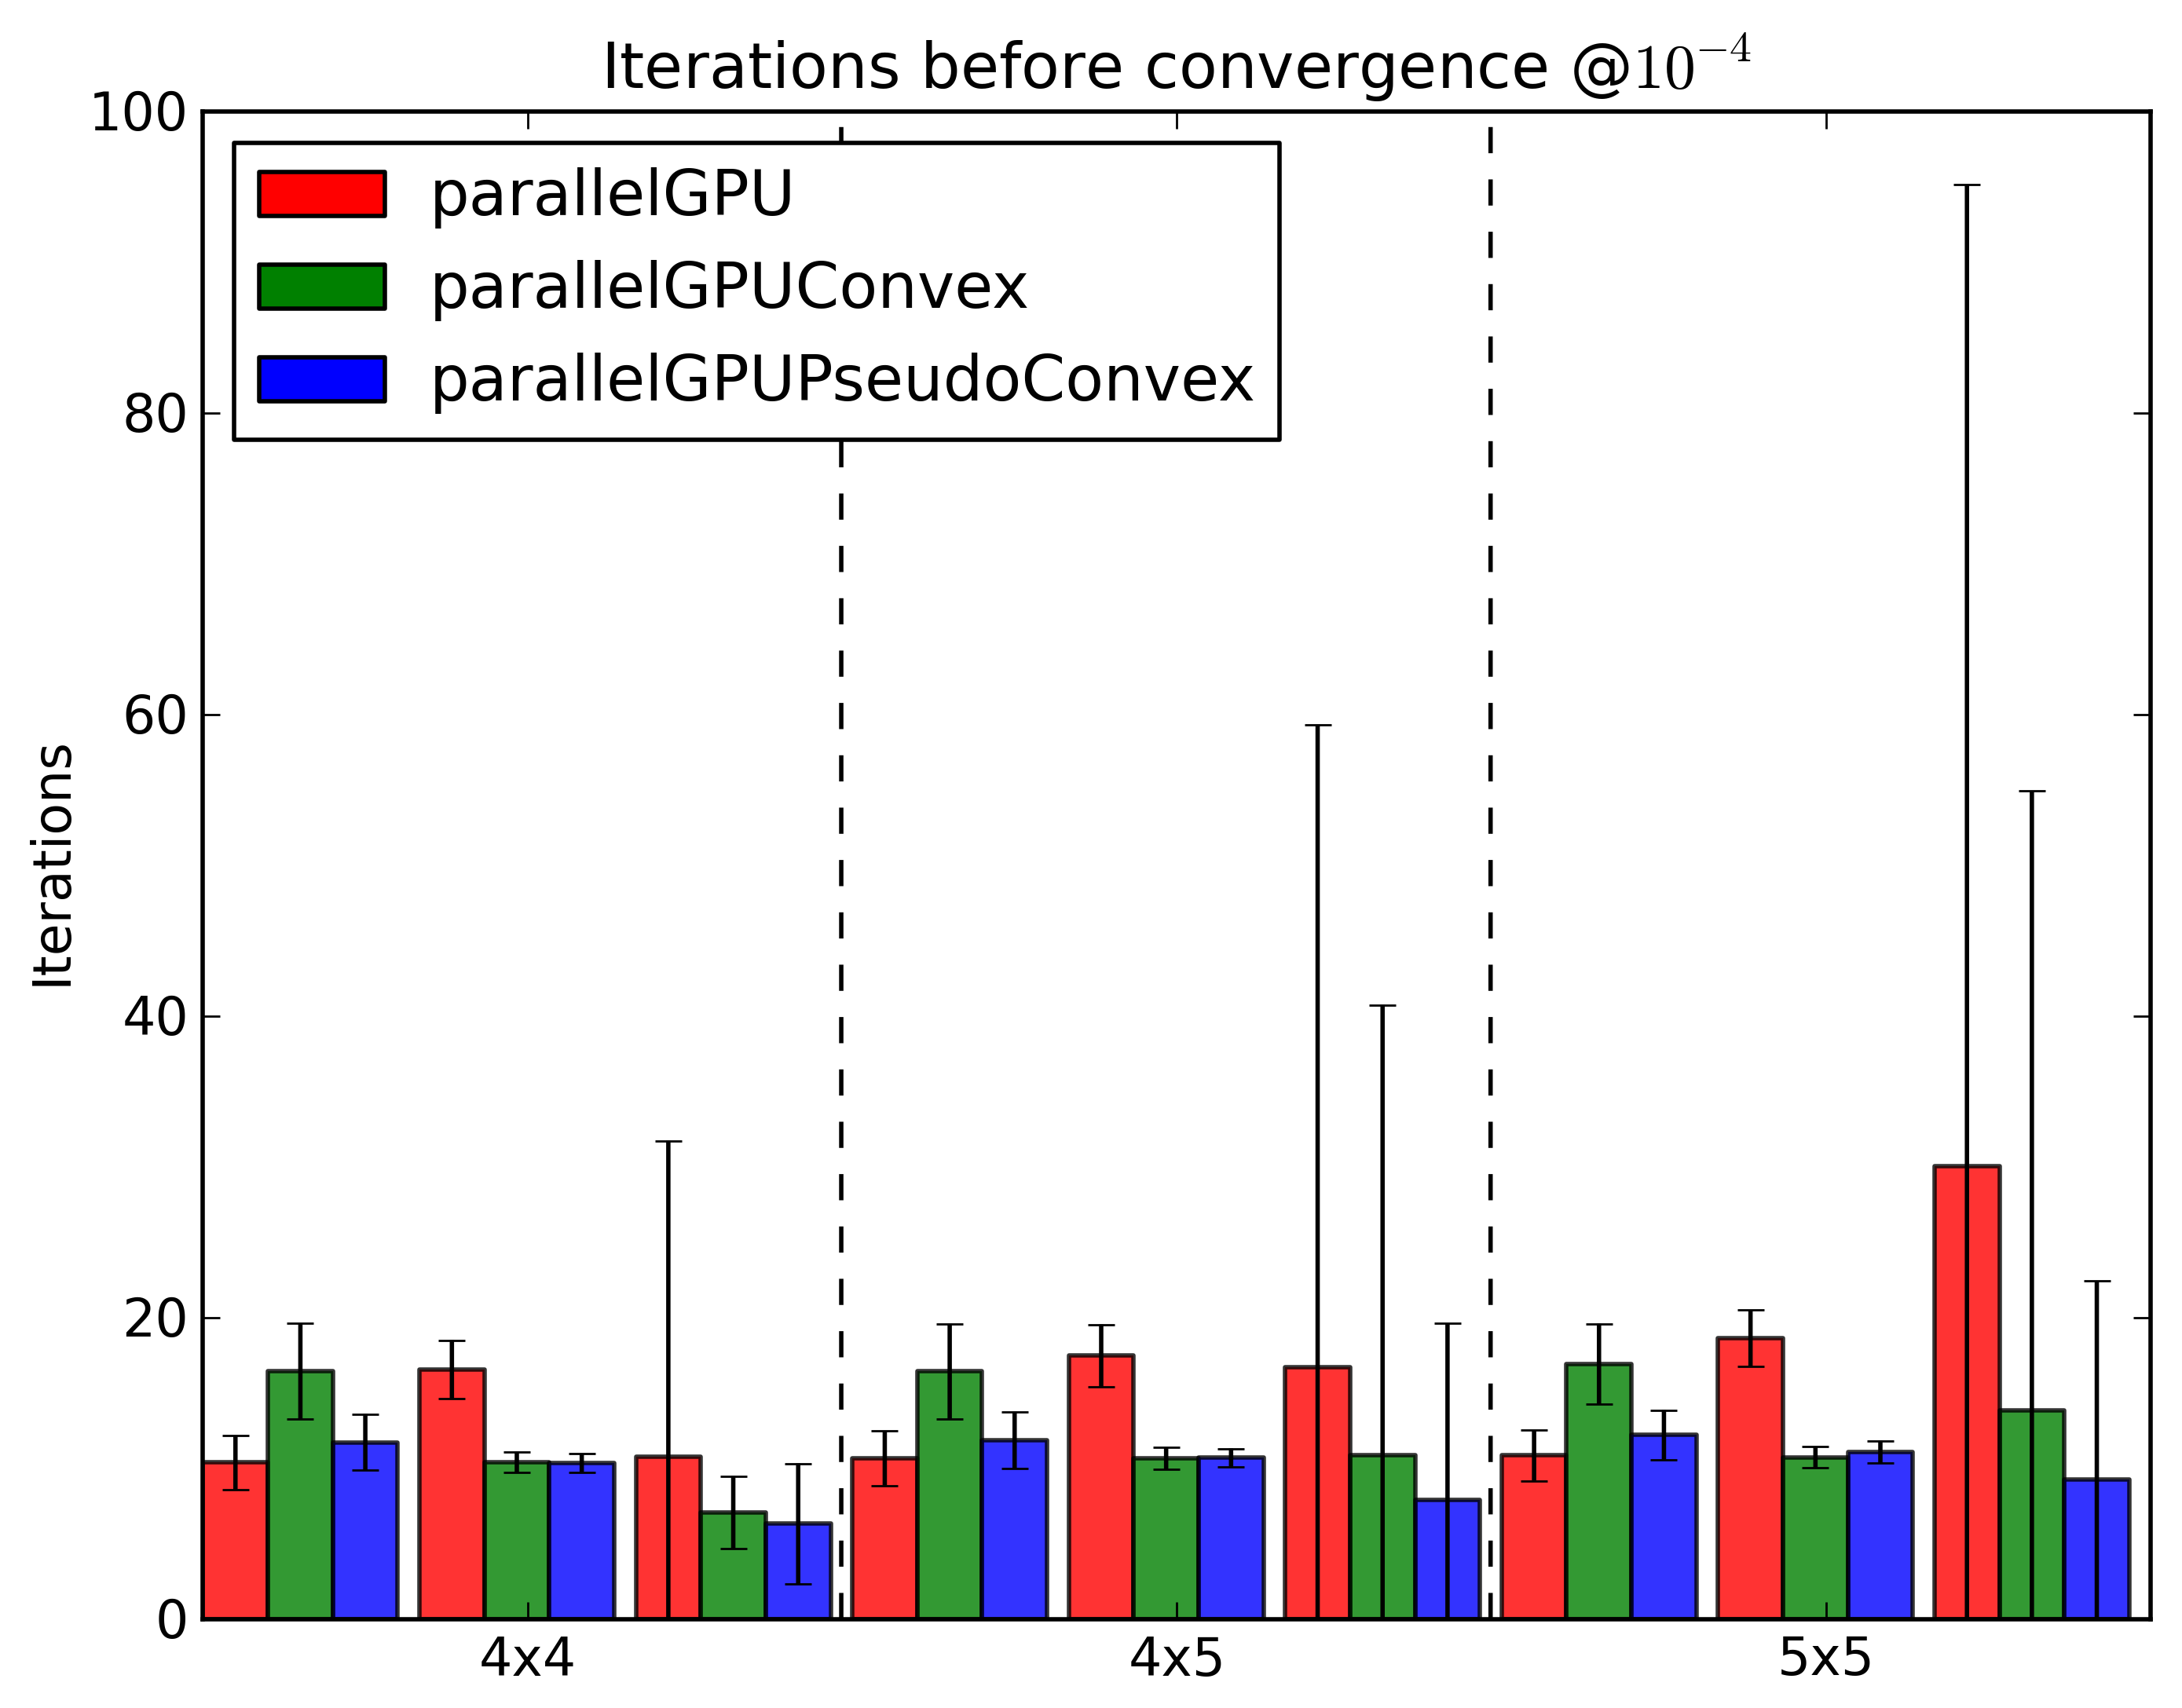
\includegraphics[width=8cm]{plots/sizes/iterations_before_convergence_e-4.png}}
	\subfigure[Accuracy]{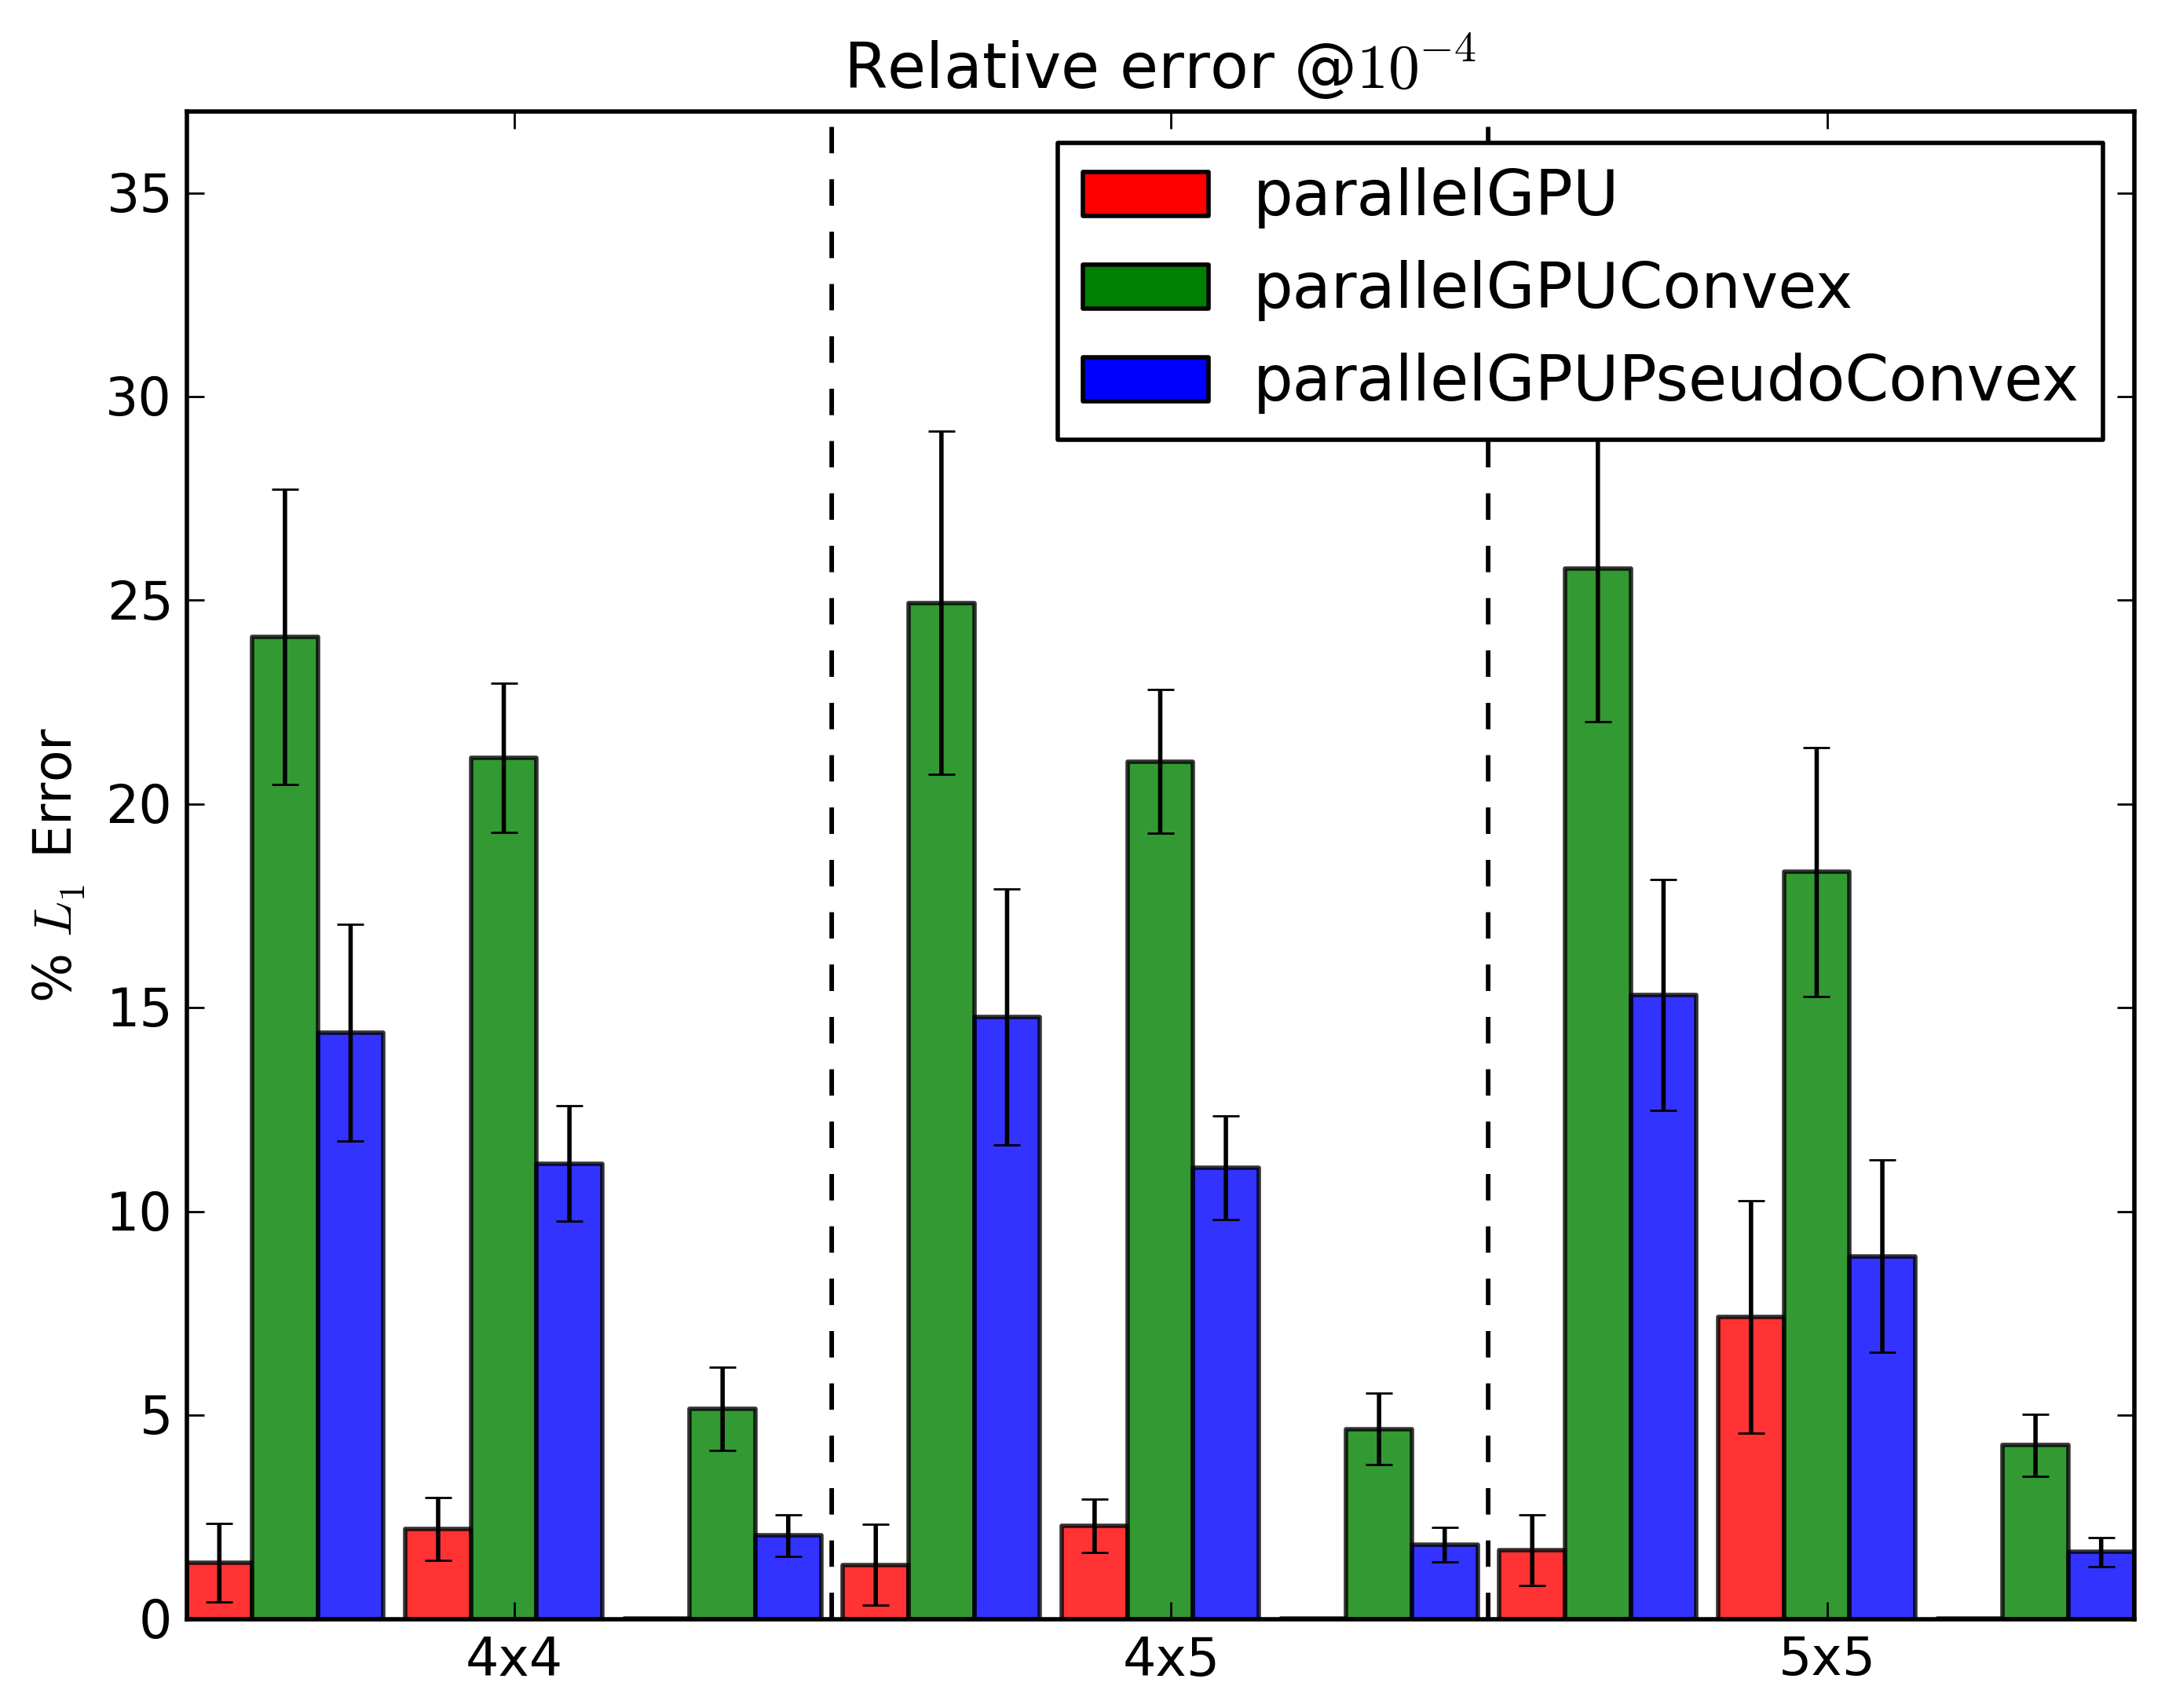
\includegraphics[width=8cm]{plots/sizes/relative_error_e-4.png}}
	\caption{Convergence and accuracy measures over $4 \times 4$, $4 \times 5$ and $5 \times 5$ models. Each group of 3 bars within a given instance size respectively represent negative strongly mixed, positive strongly repulsive and positive strongly attractive instances. The convexified and pseudo-convexified EP versions do improve convergence at a significant cost in terms of accuracy with respect to the naive parallel EP.}
	\label{444555}
\end{figure}

Using these three families of instances, we explore how convergence and accuracy is affected by the model size. Figure \ref{444555} shows the convergence and accuracy data for these three types across 3 increasing model sizes. For negative strongly mixed and positive strongly repulsive, there is no significant difference in the number of iterations before convergence. On the contrary, increasing size tends to overall lead to more instability with size on positive strongly attractive cases. On the accuracy side, there is a global degradation for all the algorithms on all instances, with the noticeable exception of the positive strongly attractive case which always leads to a very accurate solution, and the positive strongly repulsive case which turns out to be significantly more difficult on 25 nodes for the vanilla EP.

Figure \ref{asympt} shows how the convergence evolves with larger instance sizes of positive strongly attractive instances. As expected, convex EP is the most stable algorithm, followed by pseudo-convex EP. In comparison, vanilla parallel EP is strongly divergent.

\begin{figure}[h!]\centering
	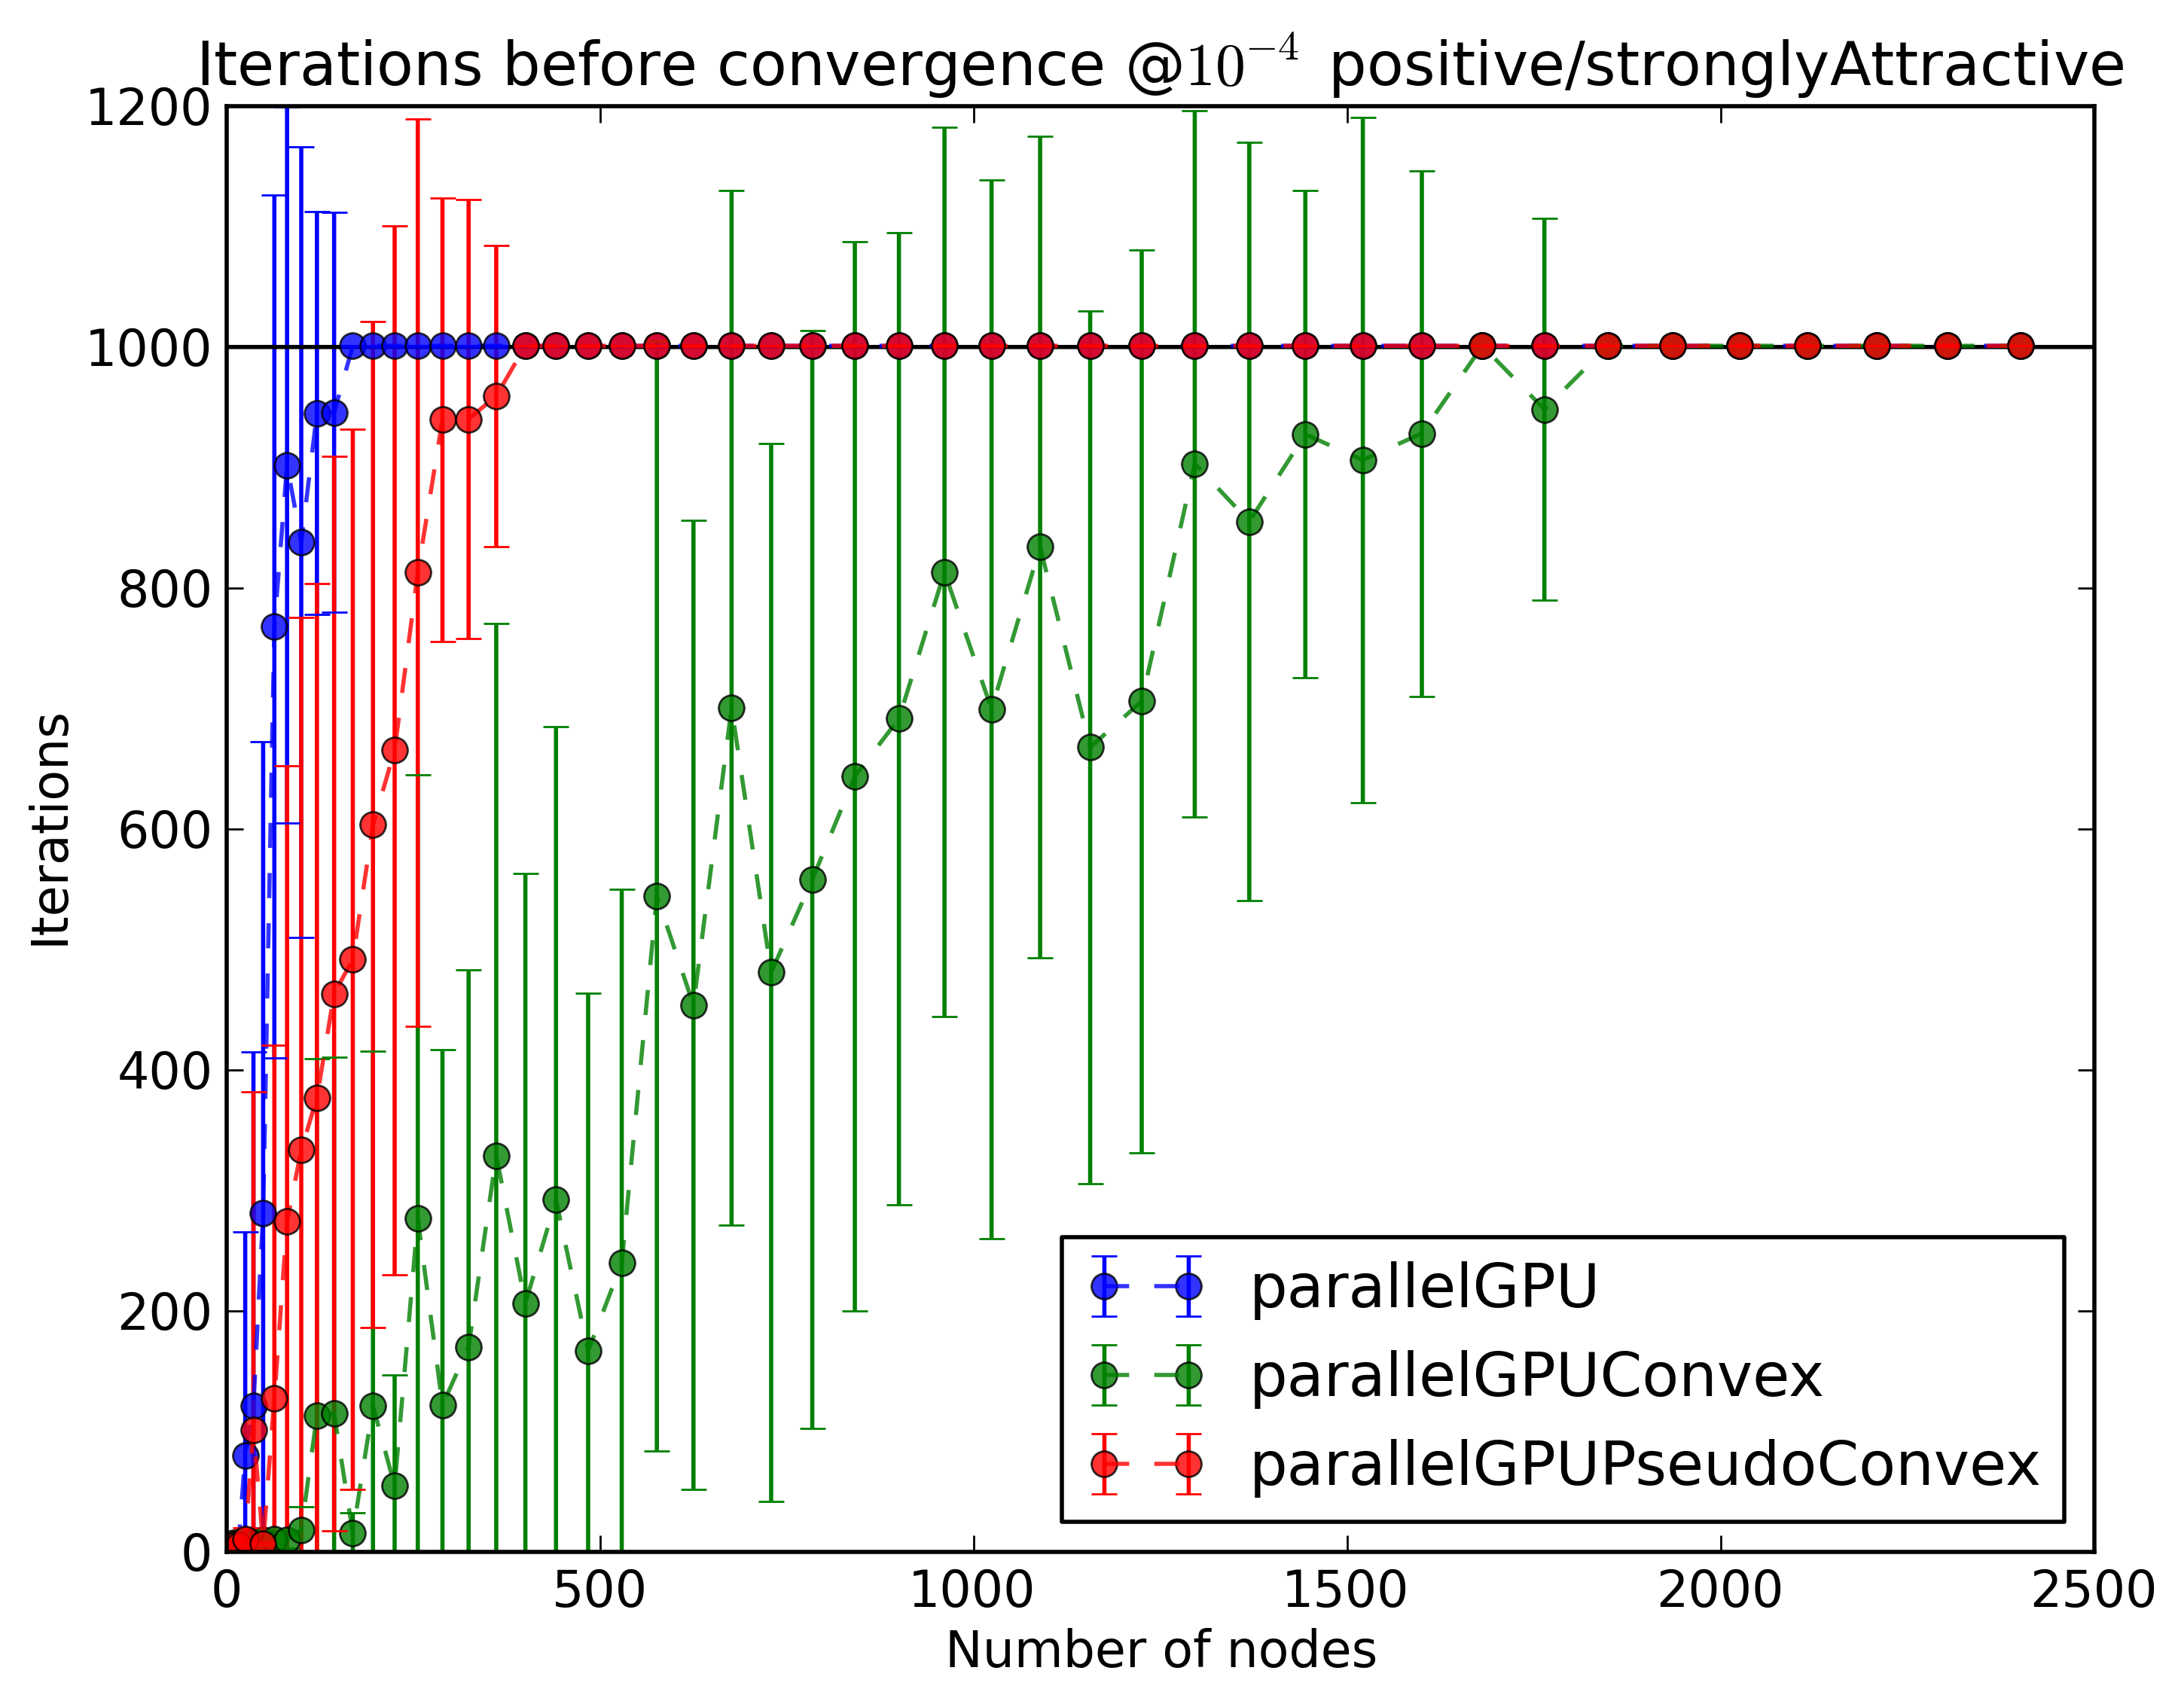
\includegraphics[width=8cm]{plots/sizes/Iterations_before_convergence_e-4_positive_stronglyAttractive.png}
	\caption{Eventually, both convex and pseudo-convex EP diverge on large positive strongly attractive instances. The maximum number of iterations was set to 1000 in this measurement.}
	\label{asympt}
\end{figure}

Last but not least, figure \ref{speed} shows how the iteration time evolves for plain sequential EP, CPU-parallelized EP and GPU-parallelized EP. The CPU parallelization becomes competitive with the sequential EP around 200 nodes instances ($15 \times 15$ Ising instances), while the larger overhead of the GPU parallelization makes it a quite effective competitor around 2000 nodes ($45 \times 45$ nodes). The bi-modal behavior of the GPU implementation for large instances is most probably due to the limited amount of on-chip memory available (256Mb). As for the smaller instances, we suspect some interference between the OS and the GPU, such as GUI rendering.

\begin{figure}[h!]\centering
	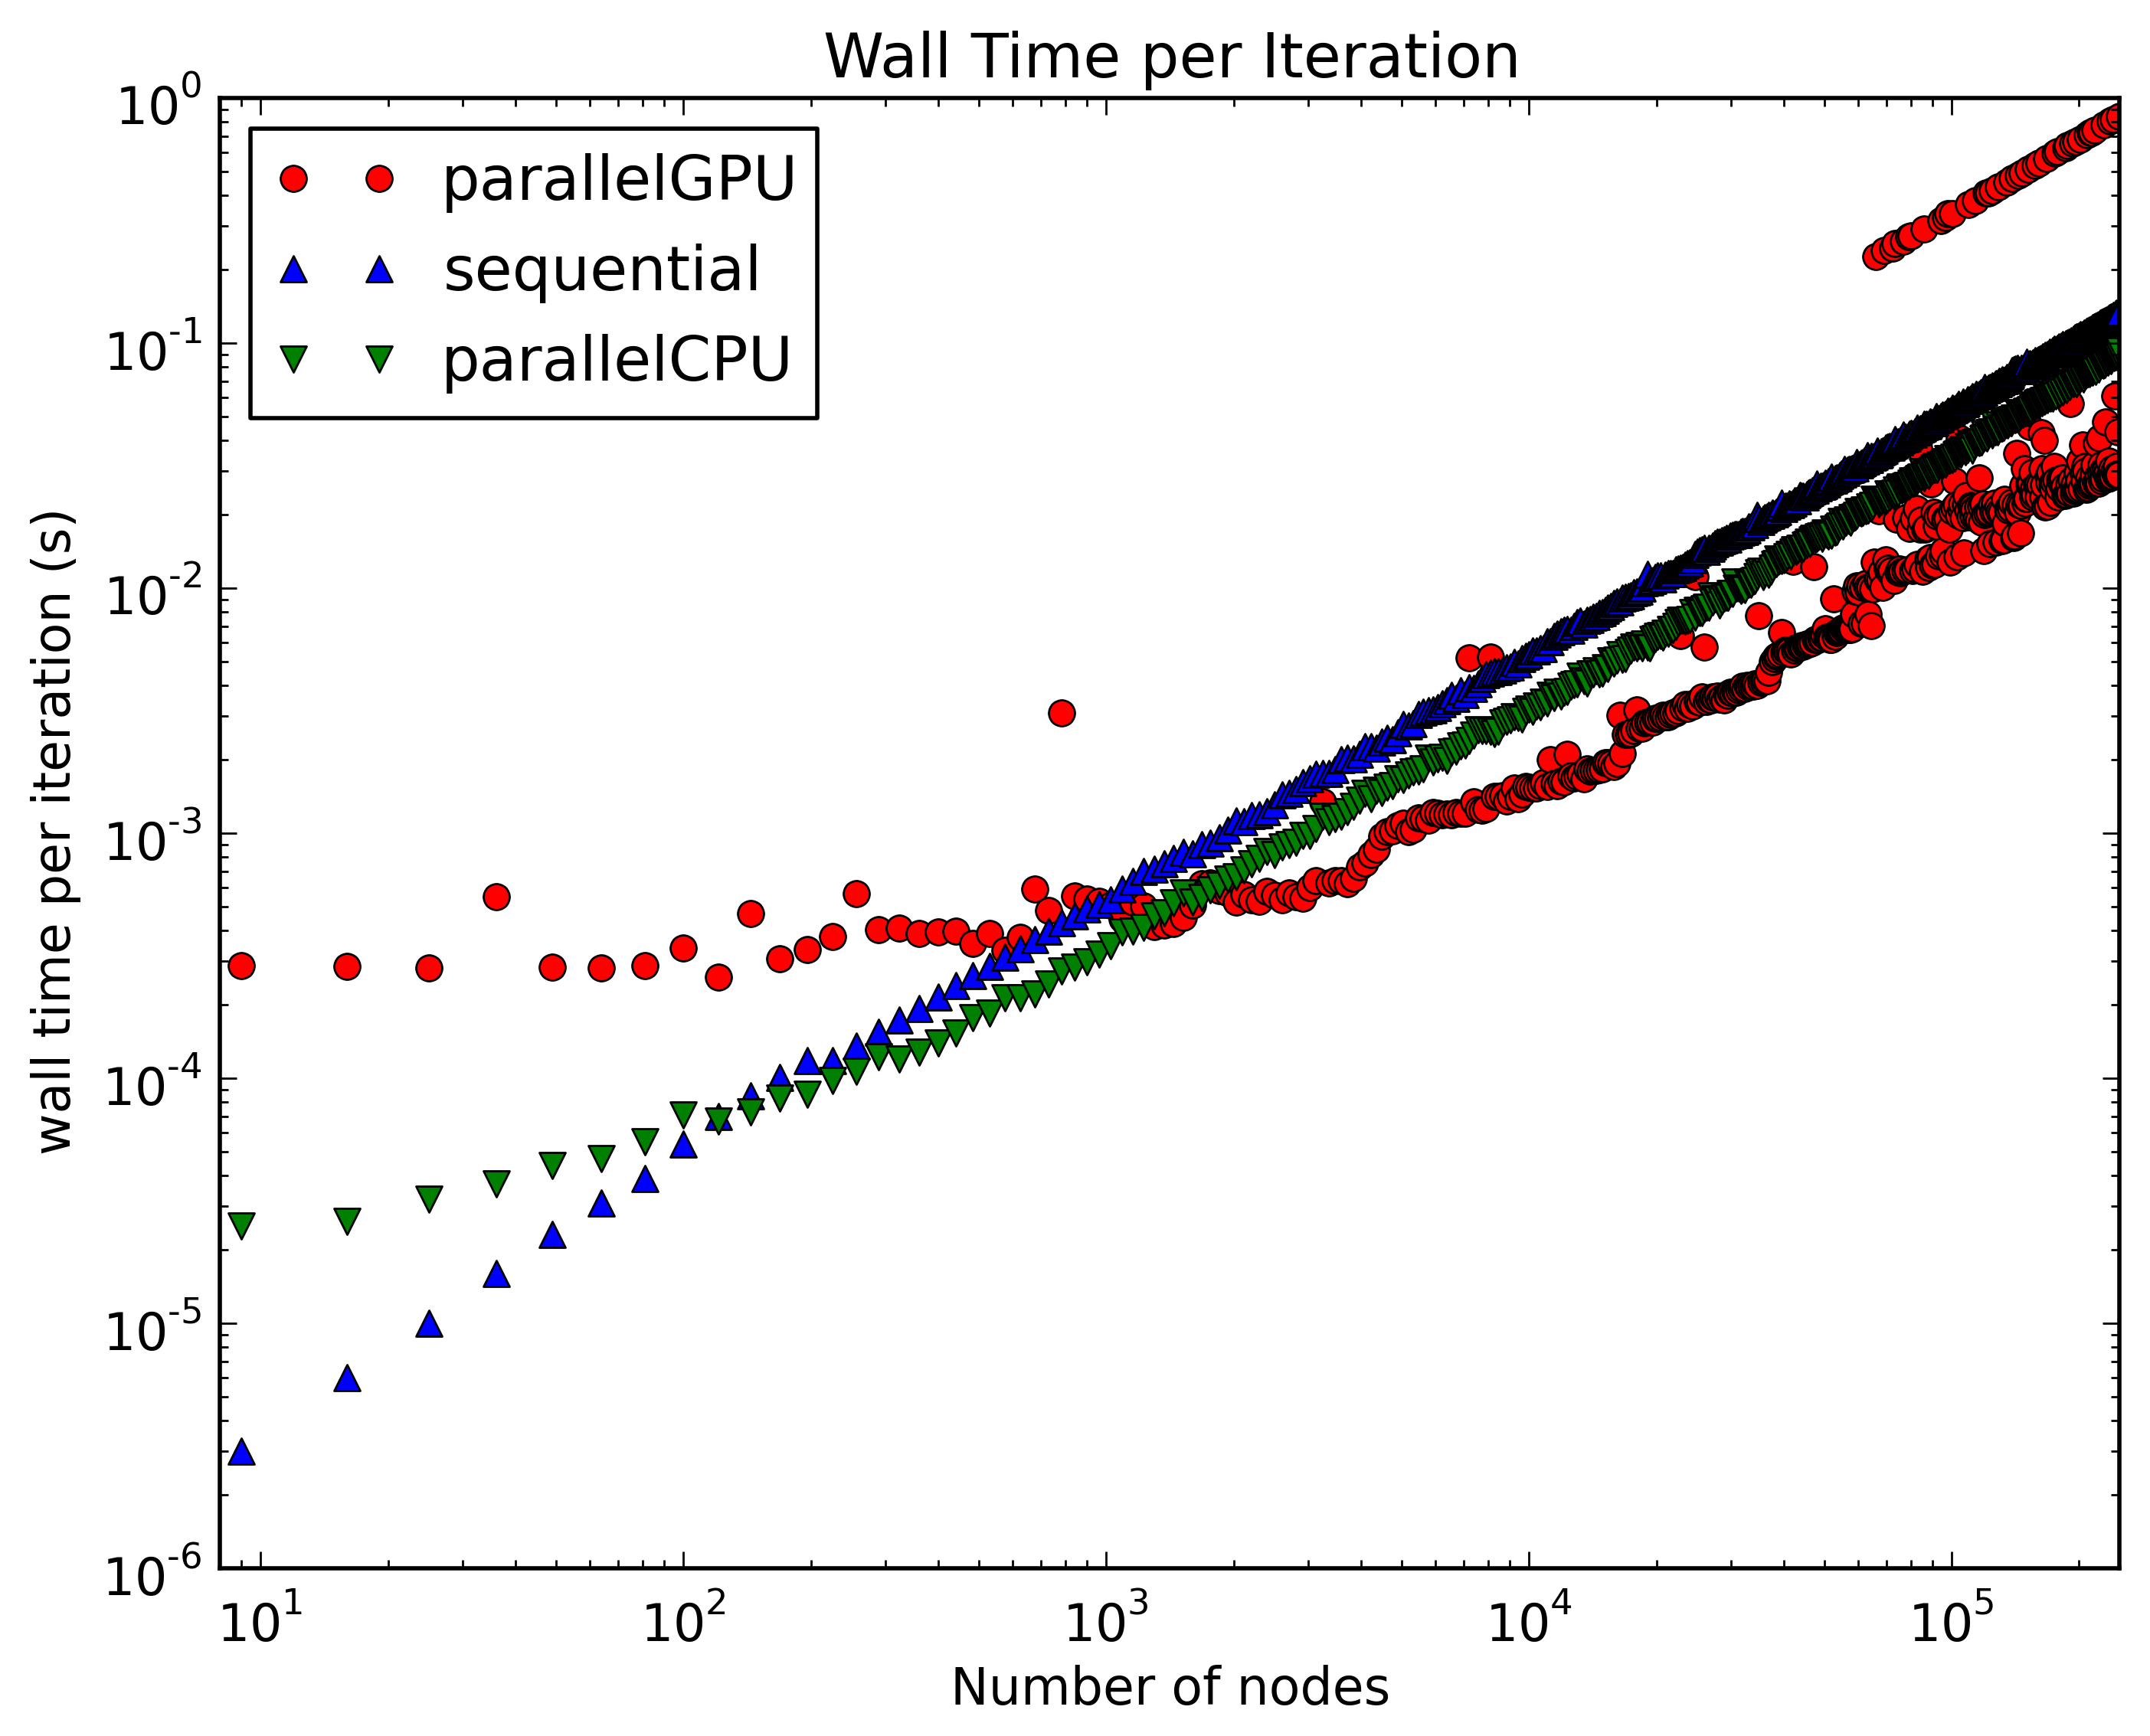
\includegraphics[width=8cm]{plots/sizes/time_per_iteration.png}
	\caption{Log-log plot of the wall time per iteration of sequential EP and parallel EPs (naive, convex and pseudo-convex) ran on a 4 cores Intel i7 CPU and a low end laptop GPU (AMD Radeon HD 6490M). Asymptotic slopes are unitary as the algorithm is linear in the number of nodes.}
	\label{speed}
\end{figure}

\section{Conclusion}
We have derived a robustified version of expectation propagation and implemented it on an OpenCL platform. The evaluation shows an improved stability for both convex and pseudo-convex expectation propagation at the cost of a decreased accuracy. The GPU implementation is only faster than sequential expectation propagation for Ising instances larger than $45 \times 45$ nodes.

There are a few natural directions for further research. First, we
can examine problems with continuous distributions like Latent
Dirichlet
Allocation~\cite{lda}. Second,
we could explore structured
approximations. For instance,
by decomposing the graph in
Figure \ref{fig:ising} into
linear chains.

\bibliographystyle{latex8}
\bibliography{refs} 

\end{document}


